\documentclass[11pt,letterpaper]{amsart}
\usepackage[headings]{fullpage} % Comment this if you use the block of fancyhdr
% ***** Language Packages *****
\usepackage[english]{babel}
%\usepackage[spanish]{babel}
\usepackage[latin1]{inputenc}
% ***** Packages for references *****
\usepackage{hyperref}
\usepackage{upref}
\usepackage{enumerate}
% ***** Packages for figures *****
\usepackage{graphicx,subfigure}
\usepackage{epsfig}
\usepackage{color}
\DeclareGraphicsExtensions{.pdf,.png,.jpg}%This command allows you to put another 
                                          %kind of files in the graphs
\usepackage{tikz}
% *** EXAMPLE ***
%\begin{figure}[ht]
%\hspace*{-2cm}\vspace*{-1cm}\includegraphics[scale=.3]
%{Homework_4_Approximations_and_exact_solution.jpg}\\
%\caption{Graph comparing the solution with the results obtained by polynomial 
% approximation.}
%\label{fgx1}
%\end{figure}
% ***** Mathematics Packages *****
\usepackage{amssymb,amsmath,latexsym,wasysym,mathrsfs,amsfonts,amsthm,bbm}
\usepackage{yfonts,amscd,amsxtra}
\usepackage{amstext,verbatim}
\usepackage{bbm}
% ***** To define margins *****
% Using geometry
\usepackage{geometry}
\geometry{left=1.5cm,right=1.5cm,top=3.5cm,bottom=2.0cm,headheight=2.3cm}
% Defining specific margins
%\setcounter{secnumdepth}{3}
%\setlength{\textheight}{190mm}
%\setlength{\textwidth}{160mm}
%\setlength{\topmargin}{-2.mm}
%\setlength{\oddsidemargin}{0mm}
%\setlength{\evensidemargin}{0mm}
%\setlength{\headheight}{0mm}
%\setlength{\headsep}{10mm}
%\setlength{\topskip}{-5mm}
%\setlength{\footskip}{20mm}
%\setlength{\parskip}{3mm plus 1mm minus 1mm}
%\setlength{\parindent}{0mm}
% ***** Packages for space between lines *****
\renewcommand{\baselinestretch}{1.2}% This is the command for the space 
                                    % between lines
% ***** Packages for tables *****
\usepackage{multicol}
\usepackage{float}
\usepackage{multirow}       %Needed for spanning rows
\restylefloat{table}
% ***** Page style with fancy headings *****
%\usepackage{fancyhdr}
%\pagestyle{fancy}
%\rhead{\bfseries Ricardo No\'e Gerardo Reyes Grimaldo\\ Oregon State University\\
%ST 563 - Theory of Statistics\\ Homework 6\\ 
%\today}
%\renewcommand{\headrulewidth}{0pt}
% ****** Packages for fonts *****
%\usepackage{txfonts}  %will make fonts slender
%\usepackage{latexsym}         %I've been using for years
%\usepackage{wasysym}          %I've been using for years
%\usepackage[pdftex]{graphicx} %I've been using for years
% ***** Package needed to insert a MATLAB paper sheet *****
%\usepackage[framed,numbered,autolinebreaks,useliterate]{mcode}
% it needs the file mcode.sty, uncomment if you need it
% *** EXAMPLE ***
% \begin{lstlisting}
% %Assignment #4
% clear all
% close all
% r=input('Tell me the initial order of the polynomial sequence ');
% q=input('Tell me the final order of the polynomial sequence ');
% Ah=.25;
% \end{lstlisting}
% ***** New commands for mathematics *****
\newcommand{\bes}{\begin{equation*}}
\newcommand{\ees}{\end{equation*}}
\newcommand{\beq}{\begin{equation}}
\newcommand{\eeq}{\end{equation}}
\newcommand{\barr}{\begin{array}}
\newcommand{\earr}{\end{array}}
\newcommand{\Pb}{\mathbb P}
\newcommand{\Prm}{\mathrm{Pr}}
\newcommand{\E}{\mathbb E}
\newcommand{\R}{\mathbb R}
\newcommand{\Q}{\mathbb Q}
\newcommand{\N}{\mathbb N}
\newcommand{\Z}{\mathbb Z}
\newcommand{\C}{\mathbb C}
\newcommand{\la}{\langle}
\newcommand{\ra}{\rangle}
\newcommand{\mA}{\bf A}
\newcommand{\mB}{\bf B}
\newcommand{\mC}{\bf C}
\newcommand{\ve}{\varepsilon}
\newcommand{\dl}{\delta}
\newcommand{\rar}{\rightarrow}
\newcommand{\lra}{\longrightarrow}
\newcommand{\Rar}{\Rightarrow}
\newcommand{\Lra}{\Longrightarrow}
\newcommand{\oo}{\infty}
\newcommand{\si}{\sigma}
\newcommand{\prt}{\partial}
\newcommand{\ka}{\kappa}
\newcommand{\J}{\mathcal J}
\newcommand{\mO}{\mathcal O}
\newcommand{\D}{\mathcal D}
\newcommand{\x}{\sf x}
\newcommand{\z}{\sf z}
\newcommand{\risk}{\mathcal{R}}
\newcommand{\Hyp}{\mathscr{H}}
\newcommand{\Ls}{\mathscr{L}^2}
\newcommand{\im}{{\tt i}}
\newcommand{\epty}{\bigcirc\hspace{-2.5mm}\big\slash}
\newcommand{\diff}[2]{\frac{\mathrm {#1}}{\mathrm{#1}#2}}
\newcommand{\rl}{\mathrm{l}}
\newcommand{\rh}{\mathrm{h}}
% ***** Commands for theorems *****
\theoremstyle{plain}
\newtheorem*{lma}{Lemma}
\newtheorem*{thm}{Theorem}
\newtheorem{theorem}{Theorem}[section]
\newtheorem{lemma}[theorem]{Lemma}
\newtheorem{corollary}[theorem]{Corollary}
\newtheorem{prop}[theorem]{Proposition}
\newtheorem{cors}{Corollary}
\newtheorem{props}{Proposition}

\theoremstyle{definition}
\newtheorem*{ack}{Acknowledgments}
\newtheorem{example}[theorem]{Example}
\newtheorem{exercise}[theorem]{Exercise}
\newtheorem{defn}[theorem]{Definition}
\newtheorem*{defs}{Definition}
\theoremstyle{remark}
\newtheorem{remark}[theorem]{Remark}
\newtheorem{convention}[theorem]{Convention}
\newtheorem{statement}[theorem]{Statement}
\newtheorem{fact}[theorem]{Fact}
\newtheorem{axiom}[theorem]{Axiom}

\usepackage{pgf,tikz}
\usepackage{mathrsfs}
\usetikzlibrary{arrows}
\usepackage{dsfont}

\title[FMDV immunity]{FMDV immunity\\Estimation of antibody dynamics}
\author{Ricardo No\'e Gerardo Reyes Grimaldo}
\address{Department of Integrative Biology\\Oregon State University}
\email{reyesgrr@oregonstate.edu}

\begin{document}
%% ***** Uncomment the following block when you don't use fancyhdr *****
%\thispagestyle{fancy}
\maketitle
In the problem of simulate the dynamics of antibody levels for Foot and Mouth Disease we 
consider a Markov Process with Probability matrix given by 
\bes
P(t\mid \pmb{\theta})=\left(\barr{cc}P_\rl(t\mid t_0=0)&P_\rh(t\mid t_0=0)\\
P_\rl(t\mid t_0=1)&P_\rh(t\mid t_0=1)\earr\right)
\ees
where $P_\rh(t)=\Prm\{$High antibody levels at time $t\}$ and $P_\rl(t)=\Prm\{$Low antibody 
levels at 
time $t\}$ and $\pmb{\theta}$ is a vector of parameters. In a simplified form, we denote 
the random walk associated with the transition probability as 
\bes
P_{Y,Z}(t\mid \textbf{$\theta$})=\Prm\left\{X(s+t)=Z\mid X(s)=Y\right\}\,.
\ees
Our focus relies in the fact that antibody levels among the different SAT can be interpreted 
as a random walk within an individual. Thus, we can consider the dynamics of antibody levels 
within a cohort of animals as multiple random walks. Each individual random walk is then 
defined through the following distribution
\bes
f(x,\textbf{t})=\prod_{j=2}^TP_{x_{j-1},x_{j}}(t_j-t_{j-1}\mid\pmb{\theta})
\ees
Hence for a sample $X_1,\dots,X_n$ of water buffaloes, where the antibody dynamics are 
independent identically distributed through the distribution $f(x,\textbf{t})$ above, we 
have  that the likelihood of this arbitrary sample is given by 
\beq
L(\pmb{\theta}\mid \textbf{x},\textbf{t})=\prod_{i=1}^{n}\prod_{j=2}^{T_i}
P_{x_{i,j-1},x_{i,j}}(t_{i,j}-t_{i,j-1}\mid\pmb{\theta})\label{likelihood}
\eeq
The transition probabilities are governed through the following system of differential 
equations
\bes\begin{split}
\diff{d}{t} P_\rh(t)&=-\lambda_\rh(t)P_\rh(t)+\lambda_\rl(t)P_\rl(t)\\
\diff{d}{t} P_\rl(t)&=-\lambda_\rl(t)P_\rl(t)+\lambda_\rh(t)P_\rh(t)
\end{split}\ees
where $\lambda_\rl(t)=$hazard of moving from low to high and $\lambda_\rh(t)=$hazard of moving 
from high to low. Since $P_\rl(t)=1-P_\rh(t)$ and $\displaystyle\diff{d}{t}(P_\rh+P_\rl)(t)=0$ 
the system above can be reduced to the ordinary differential equation
\bes
\diff{d}{t}P_\rh(t)=\lambda_\rl(t)-(\lambda_\rl(t)+\lambda_\rh(t))P_\rh(t)=\eta(t)-\gamma(t)
P_\rh(t)
\ees
Let us notice that the ODE above can be solved analytically given that $\lambda_\rl(t)$ and 
$\lambda_\rh(t)$ are determined integrable functions, where the solution is then given by 
\bes
P_\rh(t)=\left(\int_{t_0}^{t}\exp\left\{\int_{t_0}^{s}\gamma(\tau)d\tau\right\}\eta(s)ds-
P_\rh(t_0)\right)\exp\left\{-\int_{t_0}^{t}\gamma(s)ds\right\}
\ees
From the solution above we can observe that the time dependency of the hazard functions 
play a critical role in the evolution of the antibody dynamics. 
Therefore, we need to assess if such functions are time dependent or not according to the 
experimental measurements. We thus compare the following two models:
\begin{center}\begin{tabular}{c||cc} 
Model&$\lambda_\rl(t)$&$\lambda_\rh(t)$\\\hline\hline
Model 1&$a$&$b$\\
Model 2&$\displaystyle\left(\frac{\alpha-\beta}{t_{end}-t_{start}}\right)t+\left(
\frac{\alpha-\beta}{t_{end}-t_{start}}t_{start}+\alpha\right)=
ct+d$&$e$\end{tabular}\end{center}
Let us notice that whenever $\alpha=\beta$ in Model 2 we reduce to Model 1; this allows us to 
compare this nested models by using the Maximum Likelihood Estimator (MLE) and design the 
following hypothesis test
\bes
H_0:\quad\alpha=\beta\qquad\mbox{v.s.}\qquad H_1:\alpha\neq\beta
\ees
We thus find the following point estimators by using the likelihood (\ref{likelihood}) 
\begin{center}
\begin{tabular}{c||ccccc}
SAT&$\hat{a}_{MLE}$&$\hat{b}_{MLE}$&$\hat{\alpha}_{MLE}$&$\hat{\beta}_{MLE}$&$\hat{e}_{MLE}$\\
\hline\hline
SAT1&0.450635794734879&0.0932094146241297&0.669900541887672&0.146555991721188&
0.0891200968121728\\
SAT2&0.337941760897452&0.208302701098458&0.273348379072234&0.383014679455082&
0.206566595621934\\
SAT3&0.275879222040706&0.363338860591964&0.381970336932573&0.178230483666068&0.36247553412567
\end{tabular}
\end{center}
Through the use of the Likelihood Ratio Test (LRT) we can conclude that there is strong 
statistical evidence to reject the null hypothesis for the cases of SAT1 and SAT2; whilst the 
test is inconclusive for SAT2. This is further confirmed through the use of the Akaike 
Information Criterion (AIC)
\begin{center}
\begin{tabular}{c||cccc}
SAT&LRT&AIC Model 1& AIC Model 2& AIC comparison $\left(1-\exp\left(-\frac{|AIC1-AIC2|}{2}
\right)\right)$\\
\hline\hline
SAT1&0.992295837730399&593.816025975106&588.715041451824&0.921956761148986\\
SAT2&0.560697237082864&843.150614568539&844.552511643543&0.50388550266813\\
SAT3&0.971803995705221&932.153980922522&929.337937989104&0.755373193056843
\end{tabular}
\end{center}
Therefore, we can conclude that the model that best fits for our experimental data is Model 2
where we have time dependency on one of the hazard functions ($\lambda_\rl(t)$).

The analysis above relies on given deterministic functions and that the collected data is 
accurate. Nevertheless, this often is untrue or not completely reliable. Therefore, a Bayesian 
approach has been implemented. By assuming that Model 1 has parameters with uniform 
prior distributions and the likelihood given in (\ref{likelihood}) we sample the posterior 
distribution 
\bes
\pi(\pmb{\theta}\mid\textbf{x},\textbf{t})\propto L(\pmb{\theta}\mid\textbf{x},\textbf{t})
\ees 
through a Metropolis-Hastings (M-H) algorithm. The results of this Markov Chain Monte Carlo 
method we obtain a histogram of the posterior distribution, the Maximum A Posteriori (MAP) 
estimator of both parameters $a$ and $b$ 
that define the hazard functions $\lambda_\rl(t)$ and $\lambda_\rh(t)$ respectively, and 
the 95\% Credible intervals for these parameters.
\begin{center}
\begin{tabular}{c||ccc}
SAT&$\hat{a}_{MAP}$&$\hat{b}_{MAP}$&Acceptance rate\\
\hline\hline
SAT1&0.457494520560844&0.095045285534491&0.258433333333333\\
SAT2&0.342968101512515&0.211123981280086&0.222966666666667\\
SAT3&0.279533720894248&0.366114380812467&0.167566666666667
\end{tabular}
\end{center}
\begin{center}
\begin{tabular}{c||ccc}
SAT&Credible interval $a$&Credible interval $b$\\
\hline\hline
SAT1&(0.359614523621854,0.575163740647241)&(0.0702984658629116,0.125296240300929)\\
SAT2&(0.268534220168746,0.4322409462545)&(0.169627774260504,0.2600386418752)\\
SAT3&(0.224755918189966,0.344664924464384)&(0.299140253996511,0.449573780637181)
\end{tabular}
\end{center}
The following are some of the most representative graphical results of our different analyses. 
From the experimental data we have the following proportions of antibody dynamics among the 
different animals in the studied buffalo cohort.
\begin{center}
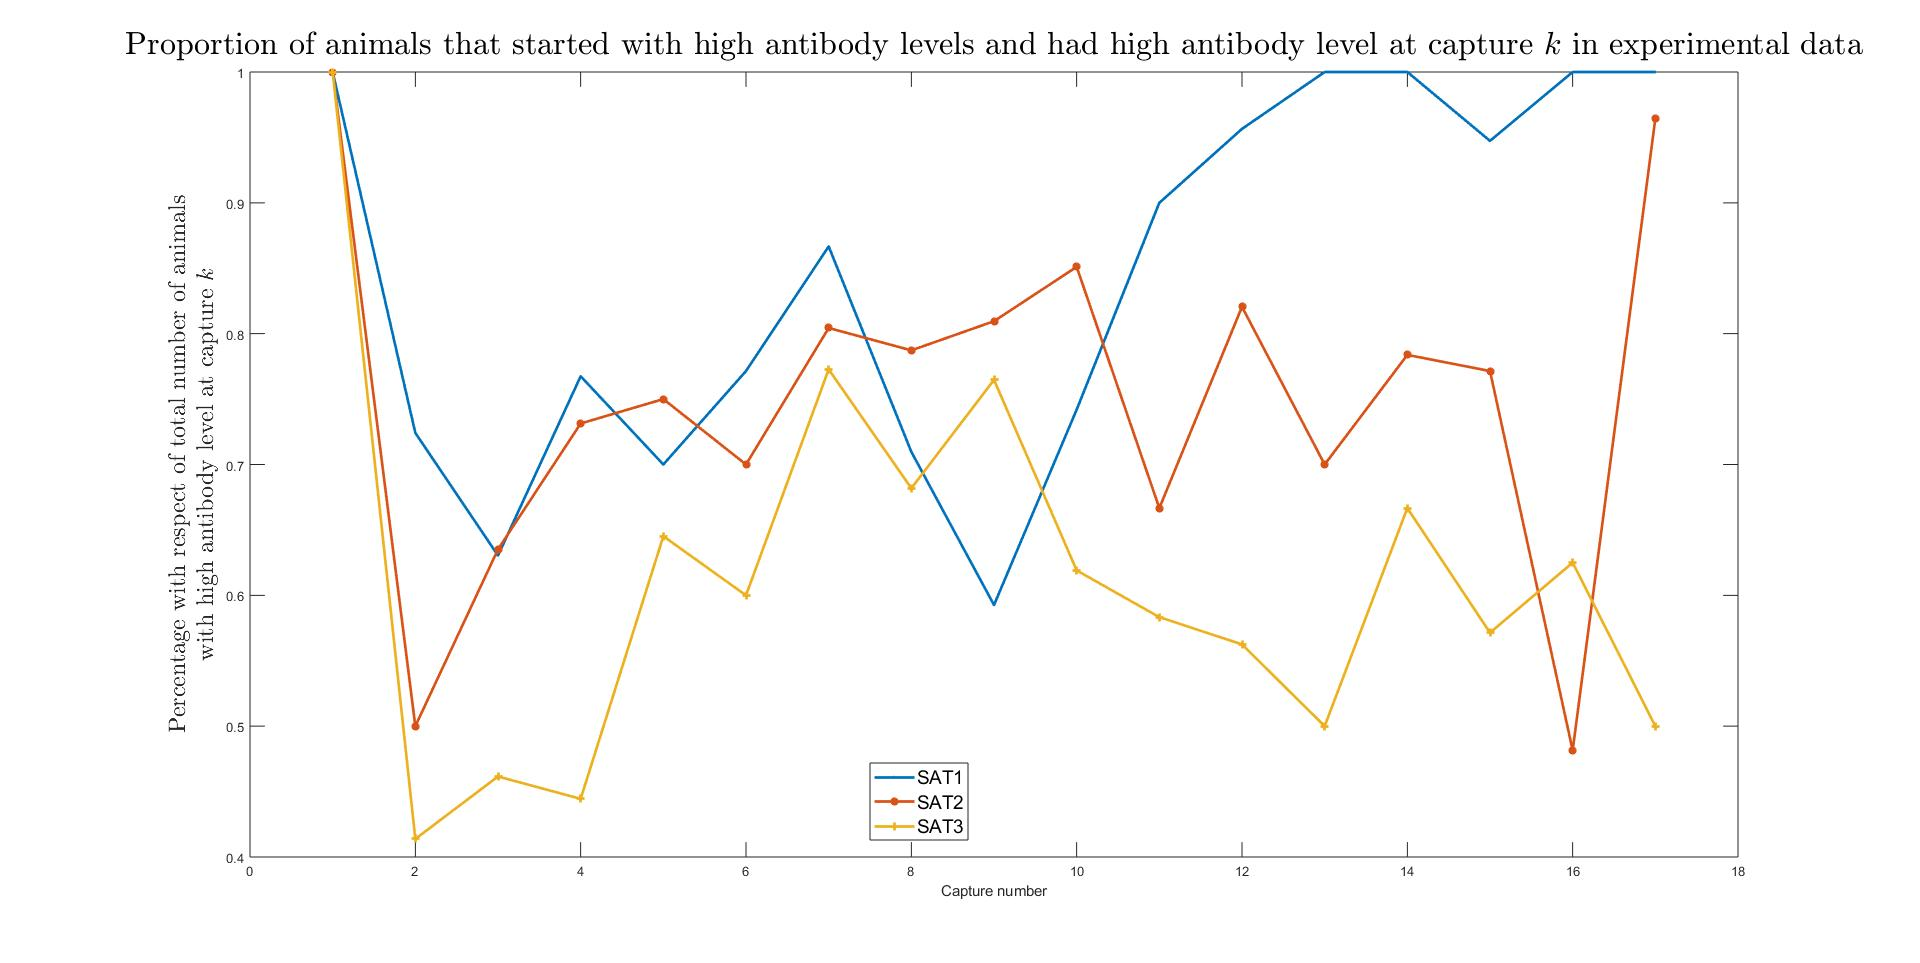
\includegraphics[width=0.4\textwidth]{12.jpg}
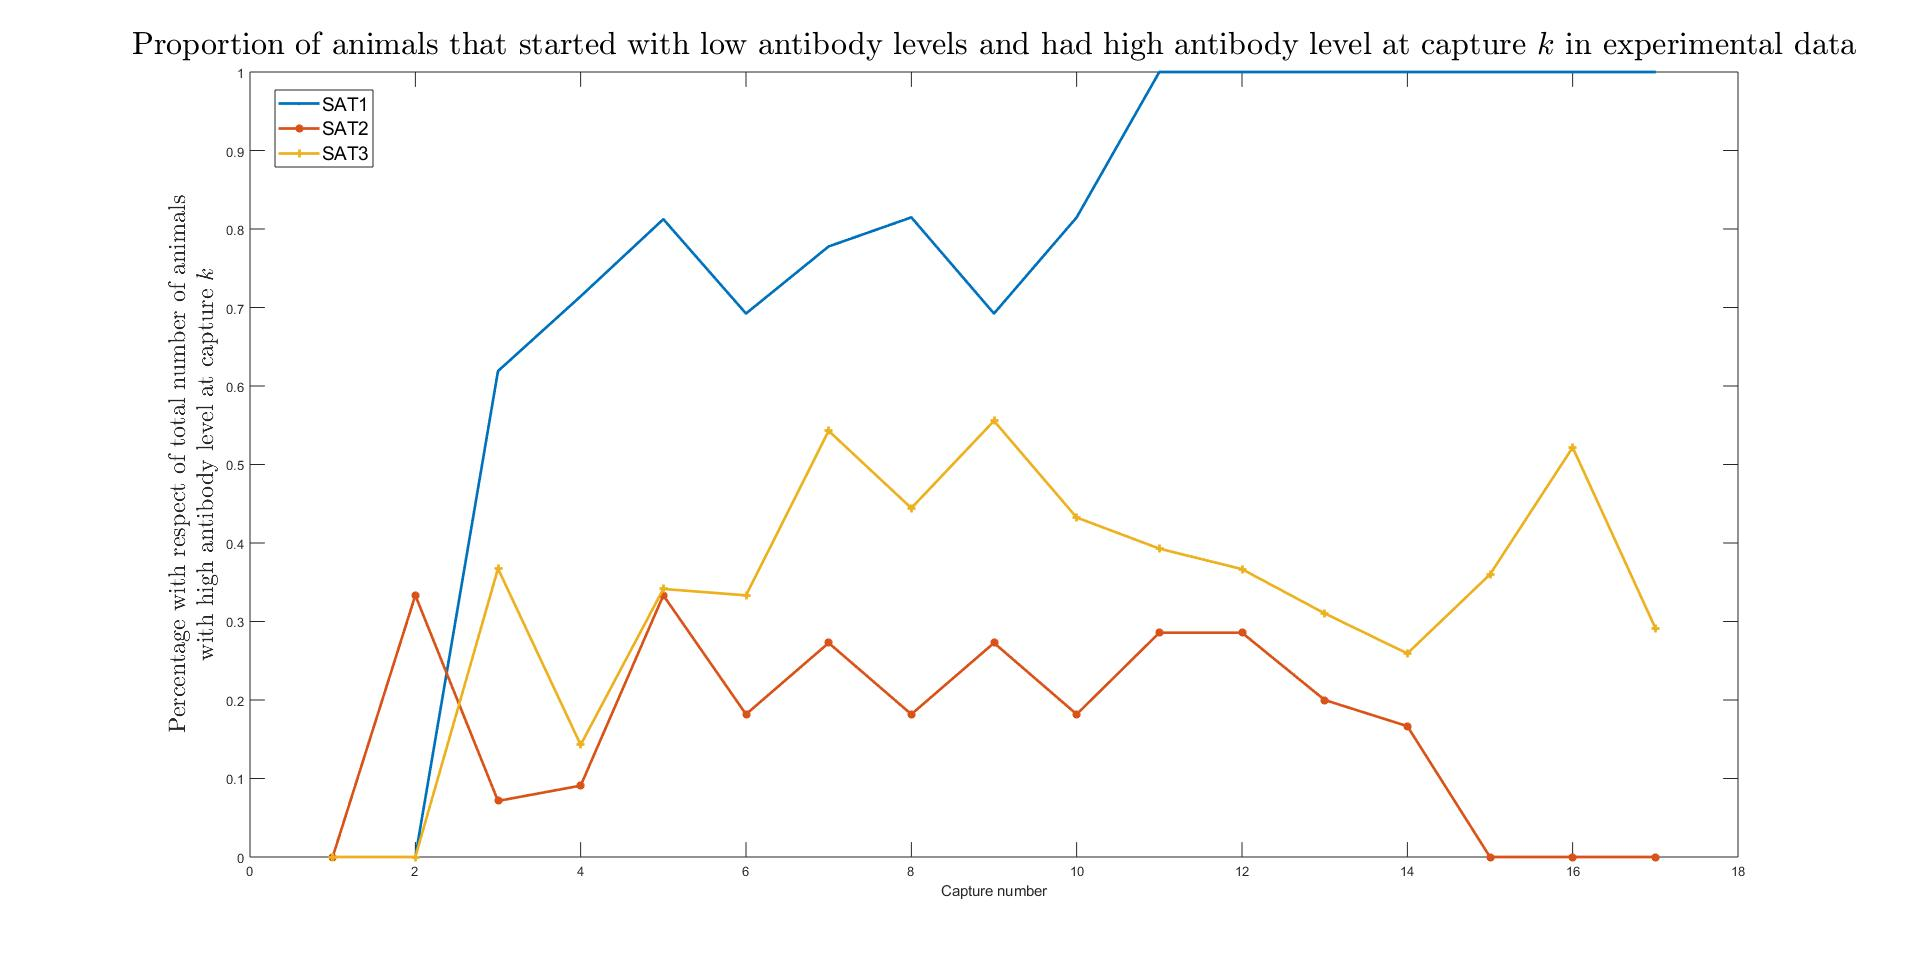
\includegraphics[width=0.4\textwidth]{13.jpg}
\end{center}
Simulating data through Model 1, by using the MLE estimator given above we obtain the following
\begin{center}
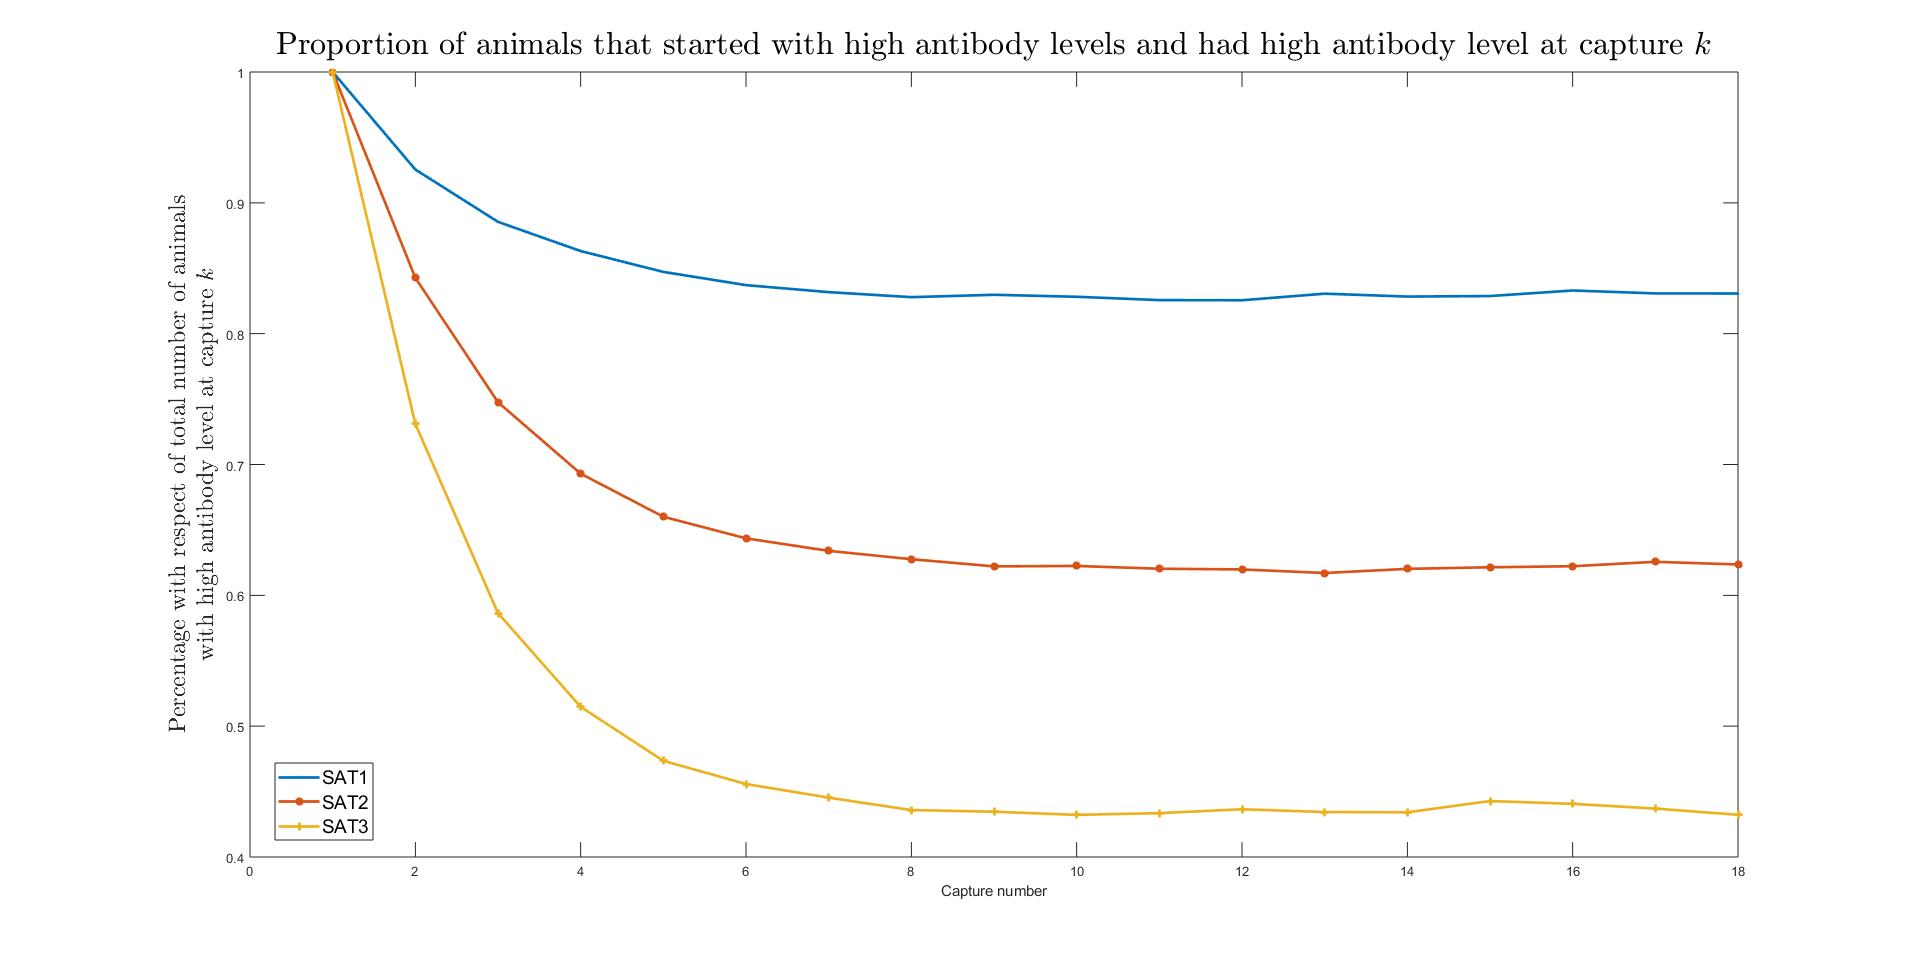
\includegraphics[width=0.4\textwidth]{fig1.jpg}
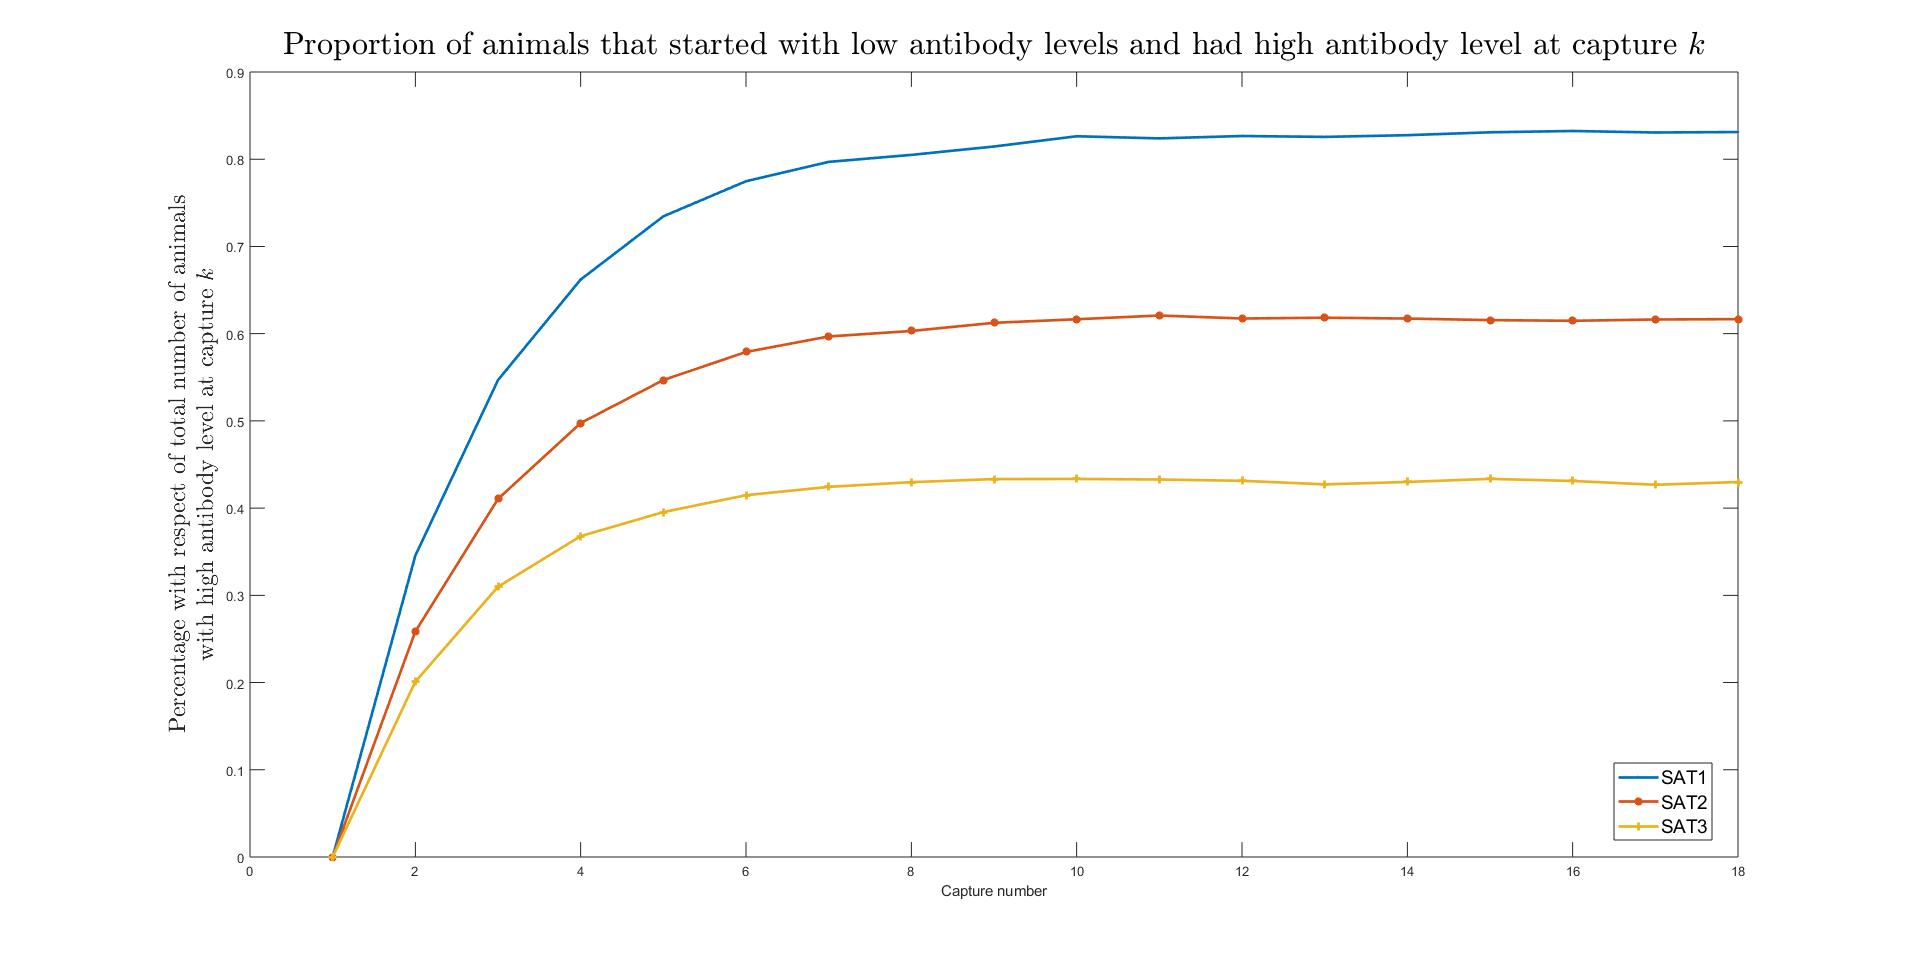
\includegraphics[width=0.4\textwidth]{fig2.jpg}
\end{center}
In contrast with the simulated data through Model 2
\begin{center}
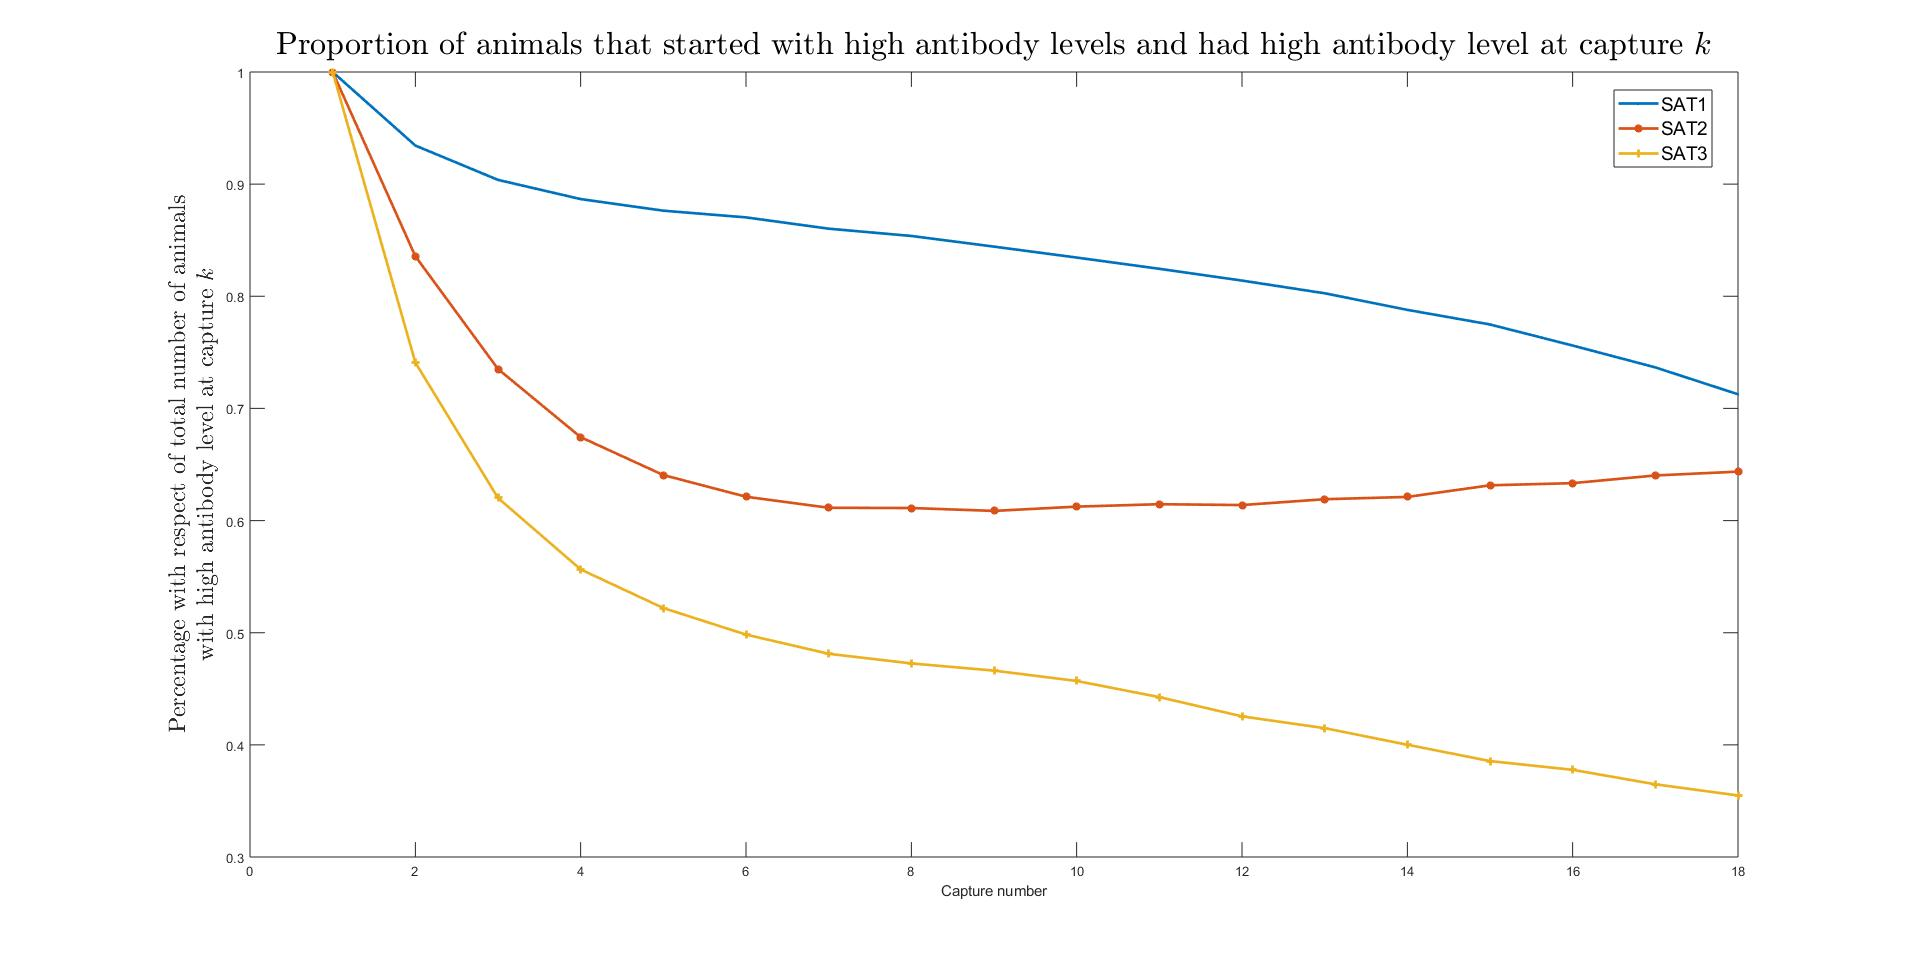
\includegraphics[width=0.4\textwidth]{fig3.jpg}
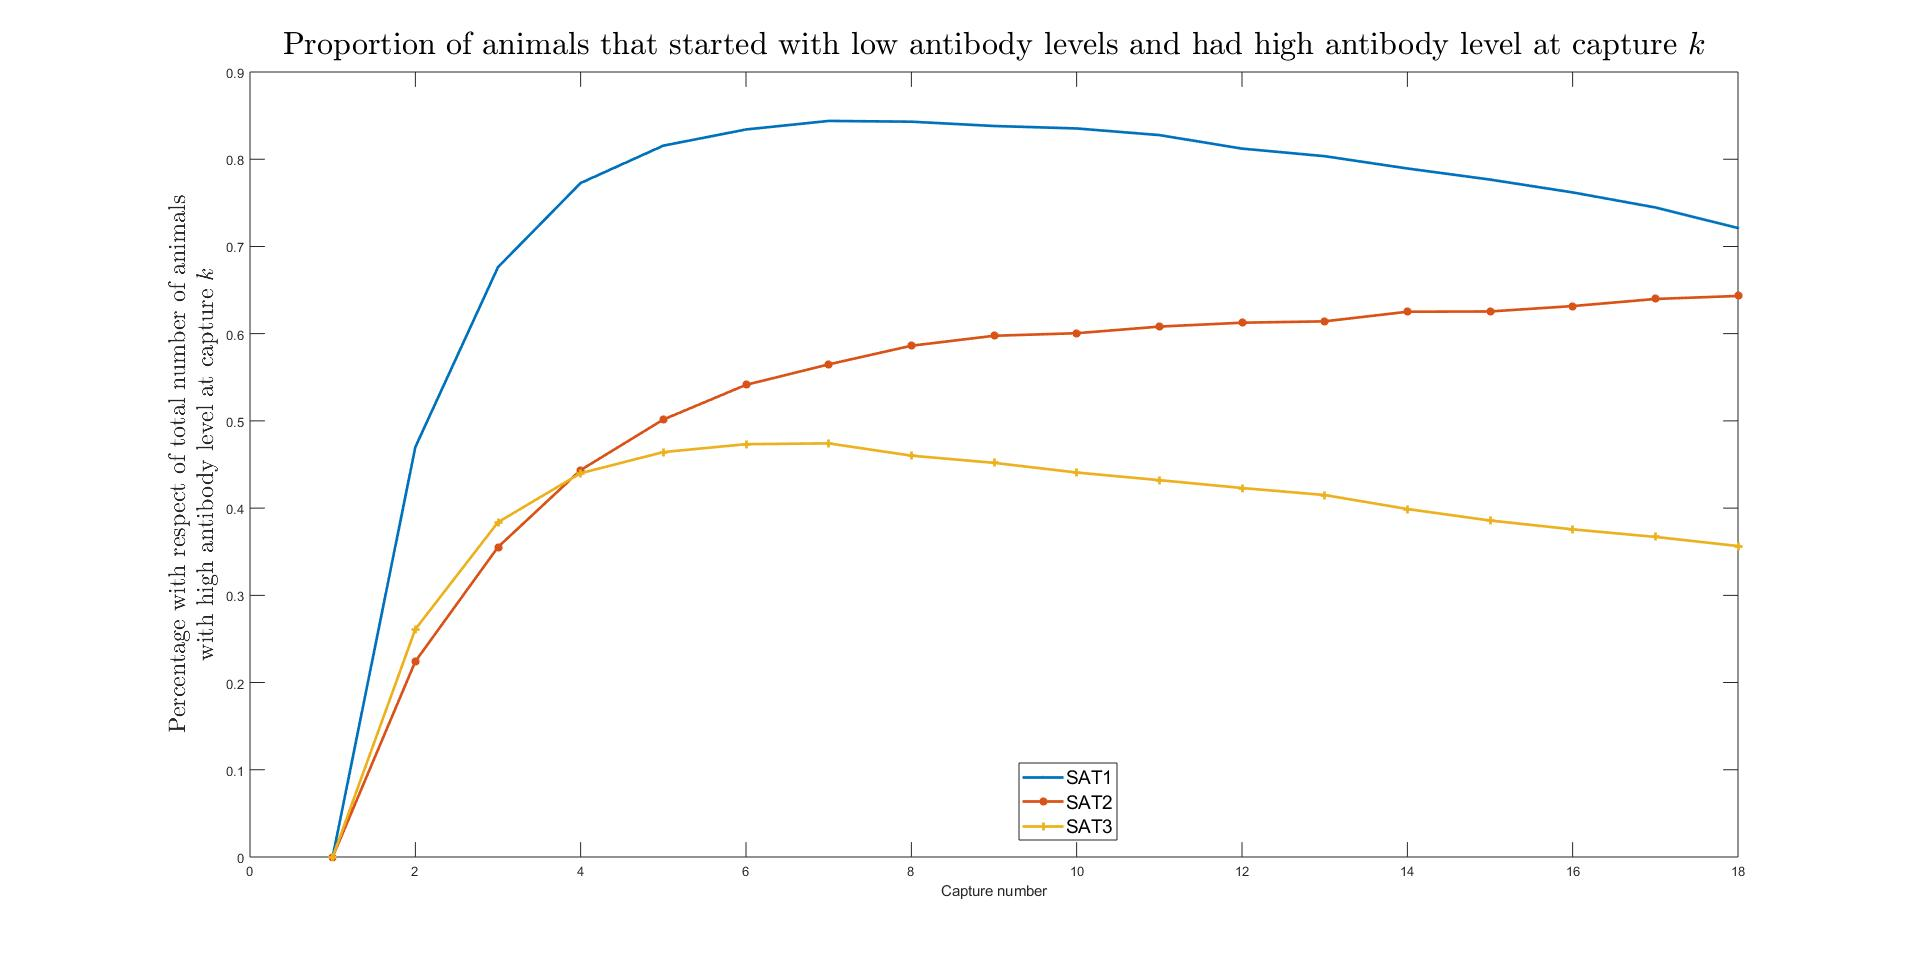
\includegraphics[width=0.4\textwidth]{fig4.jpg}
\end{center}
We then observe the coverage of these two models to the experimental data
\begin{center}
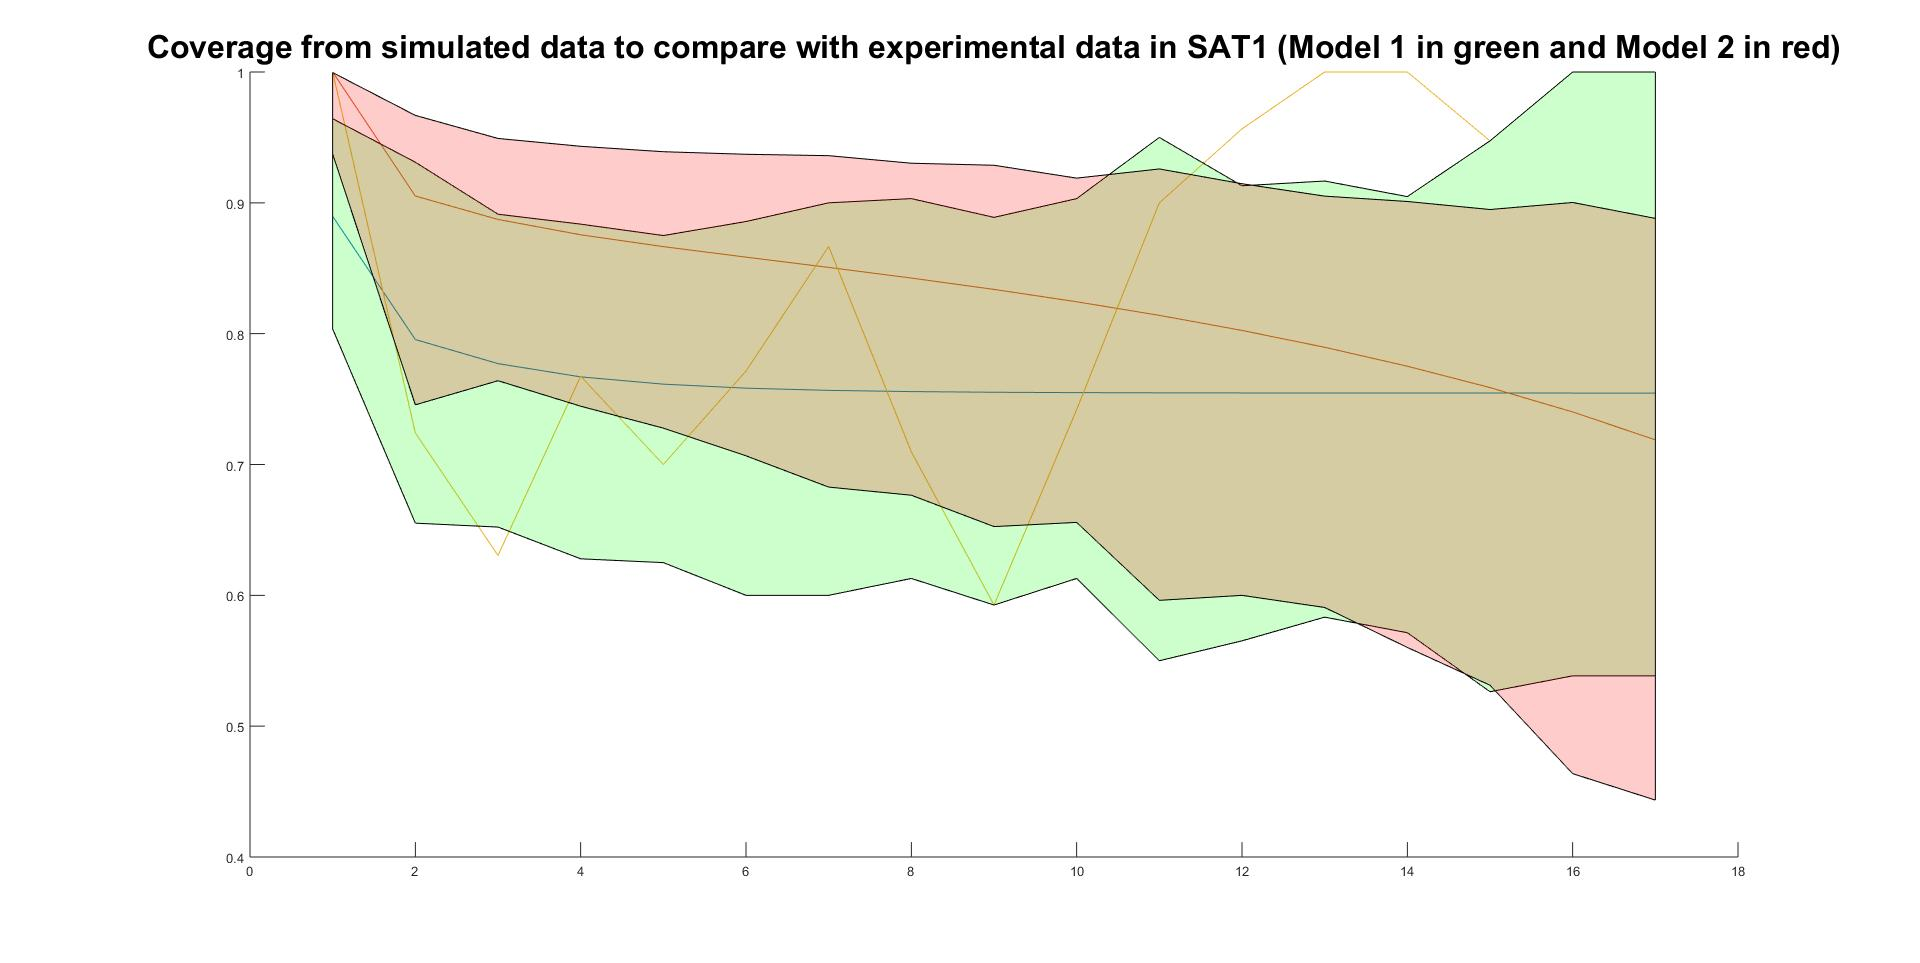
\includegraphics[width=0.4\textwidth]{fig11.jpg}
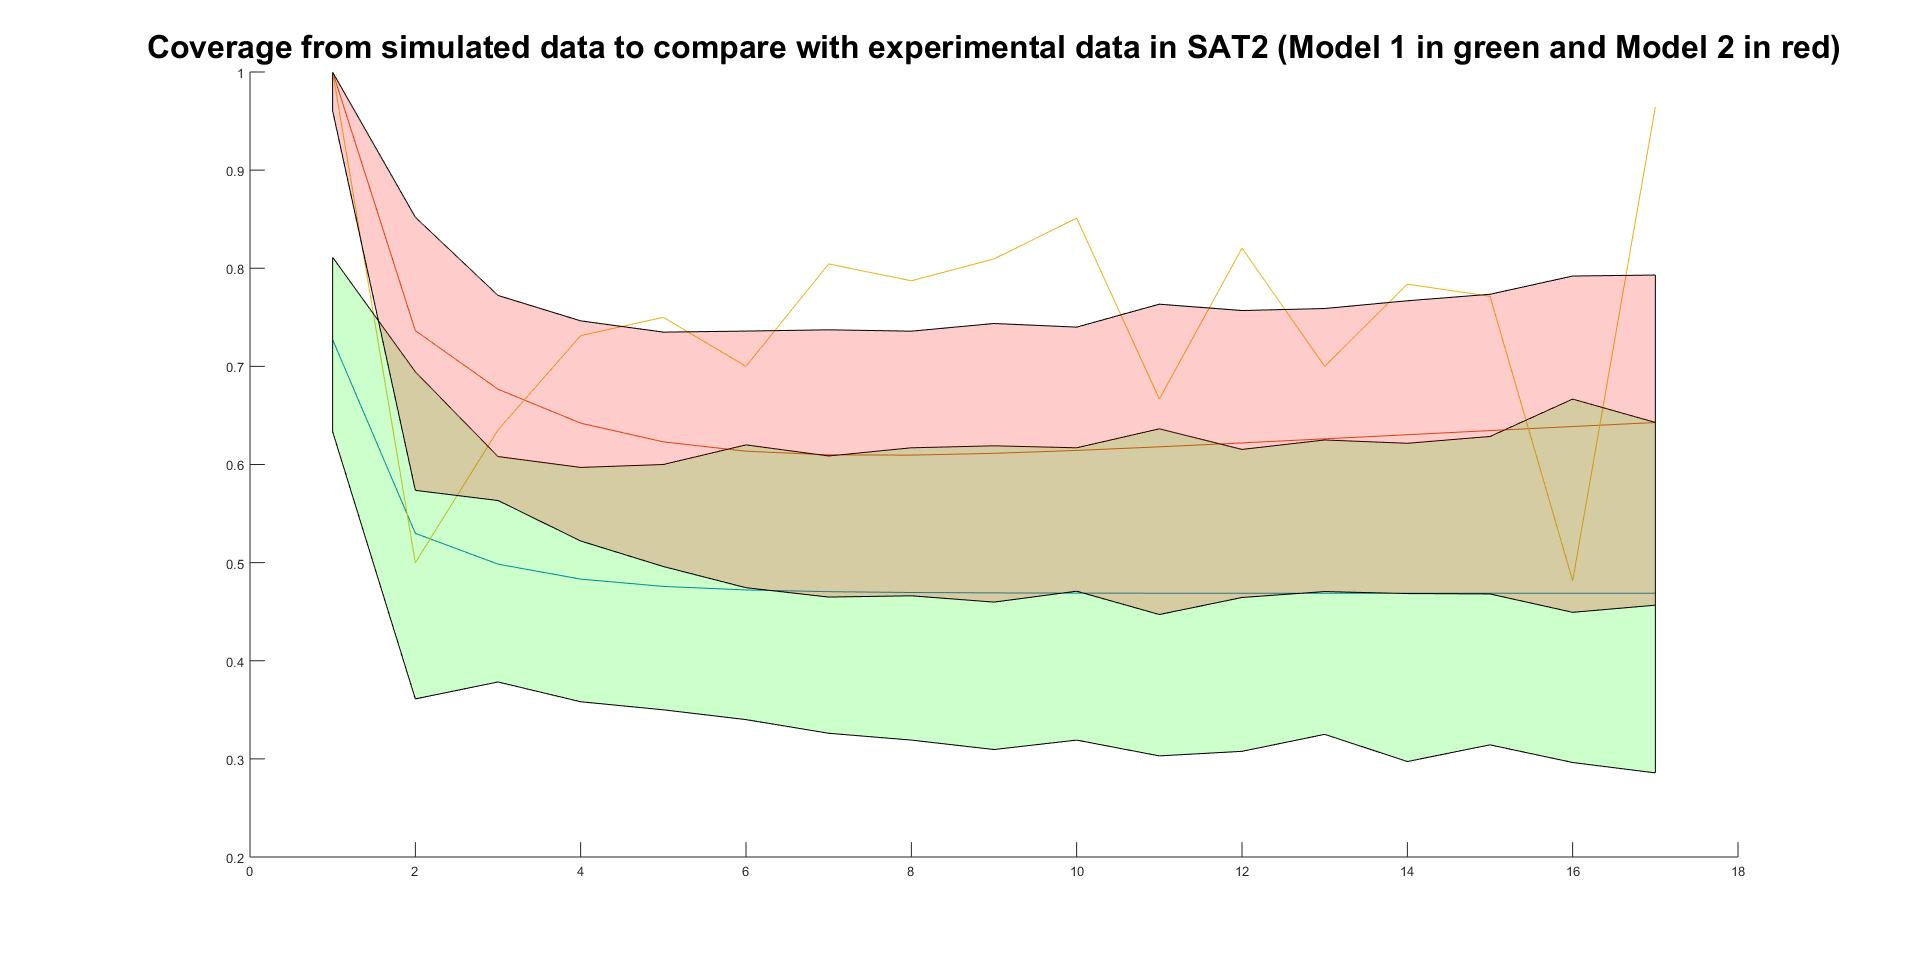
\includegraphics[width=0.4\textwidth]{fig12.jpg}
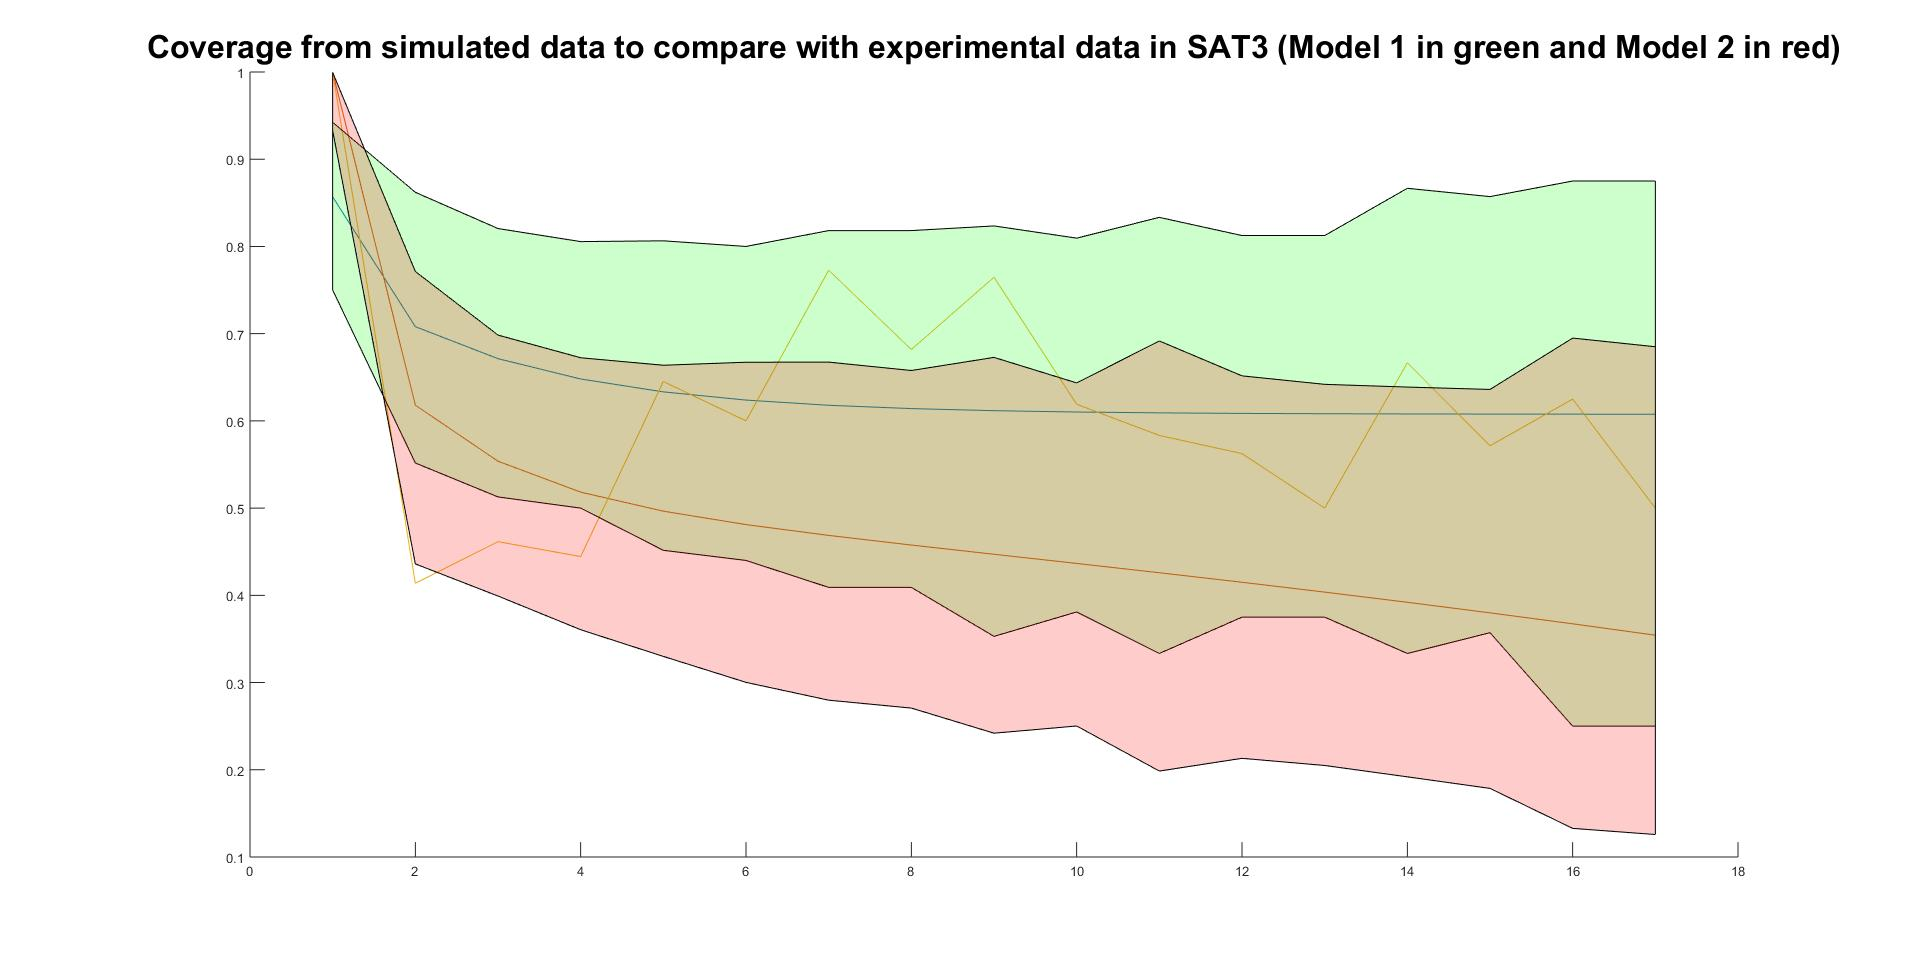
\includegraphics[width=0.4\textwidth]{fig13.jpg}
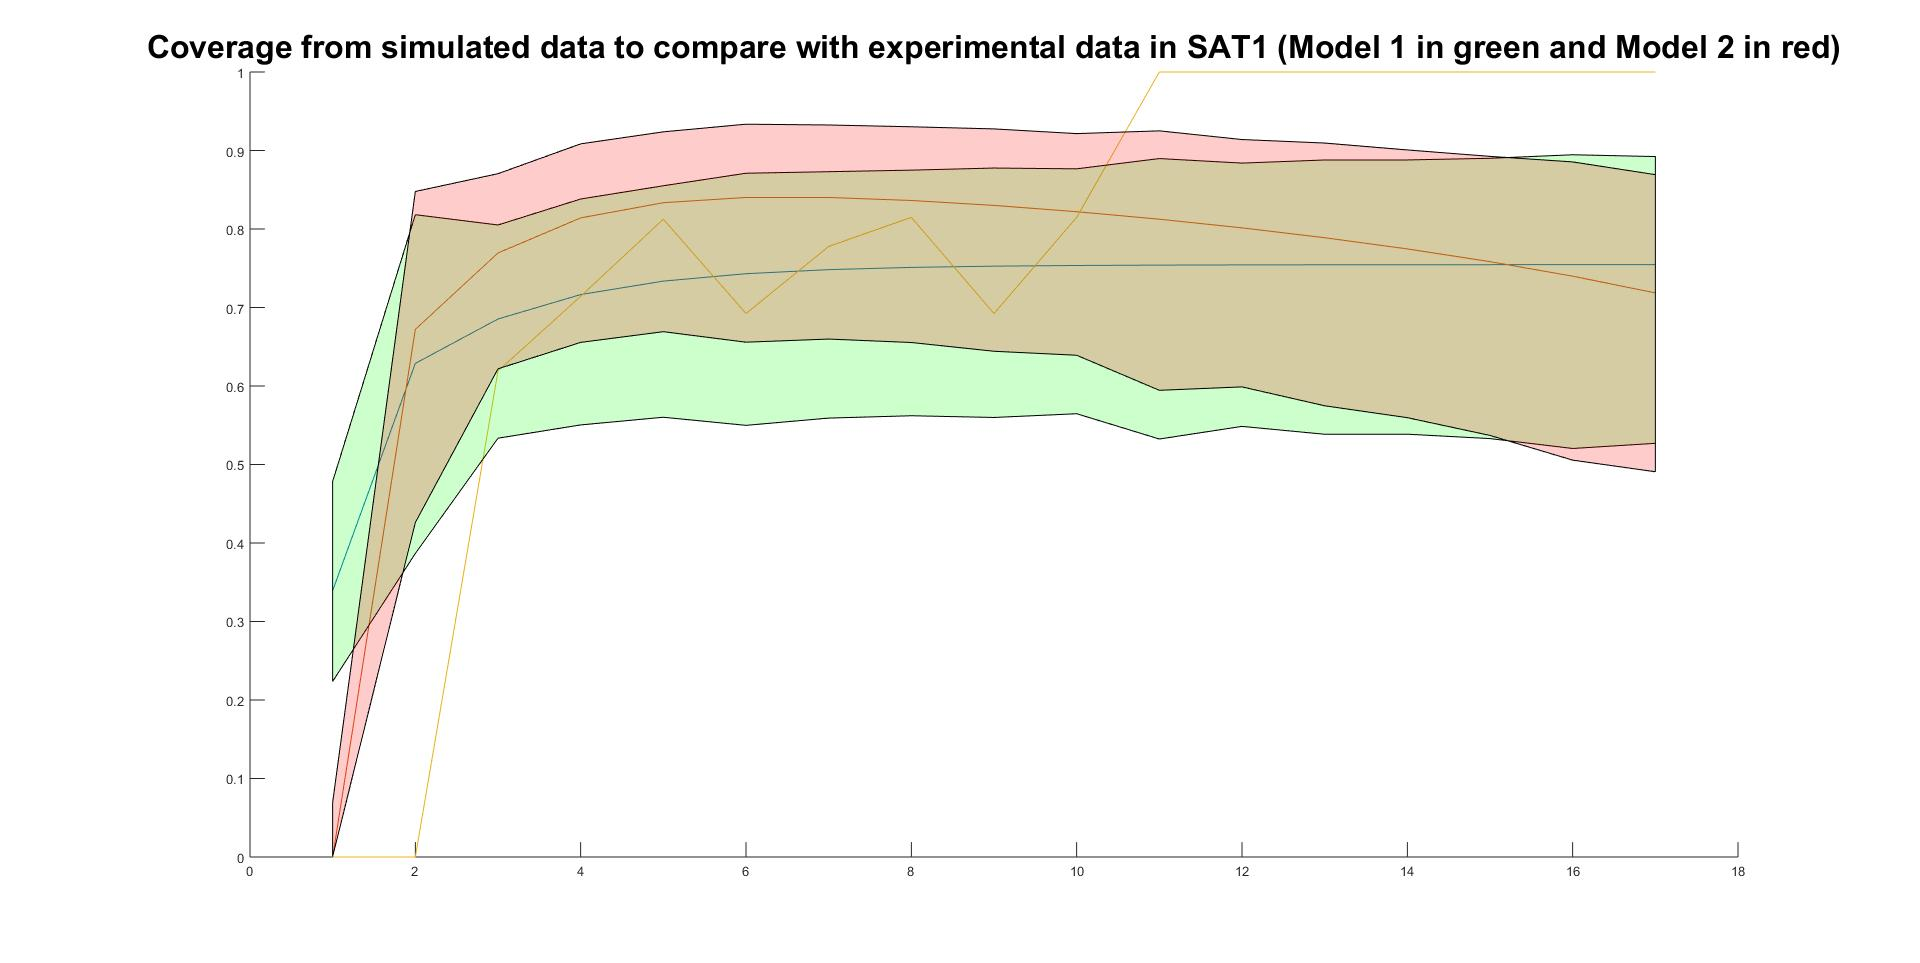
\includegraphics[width=0.4\textwidth]{fig14.jpg}
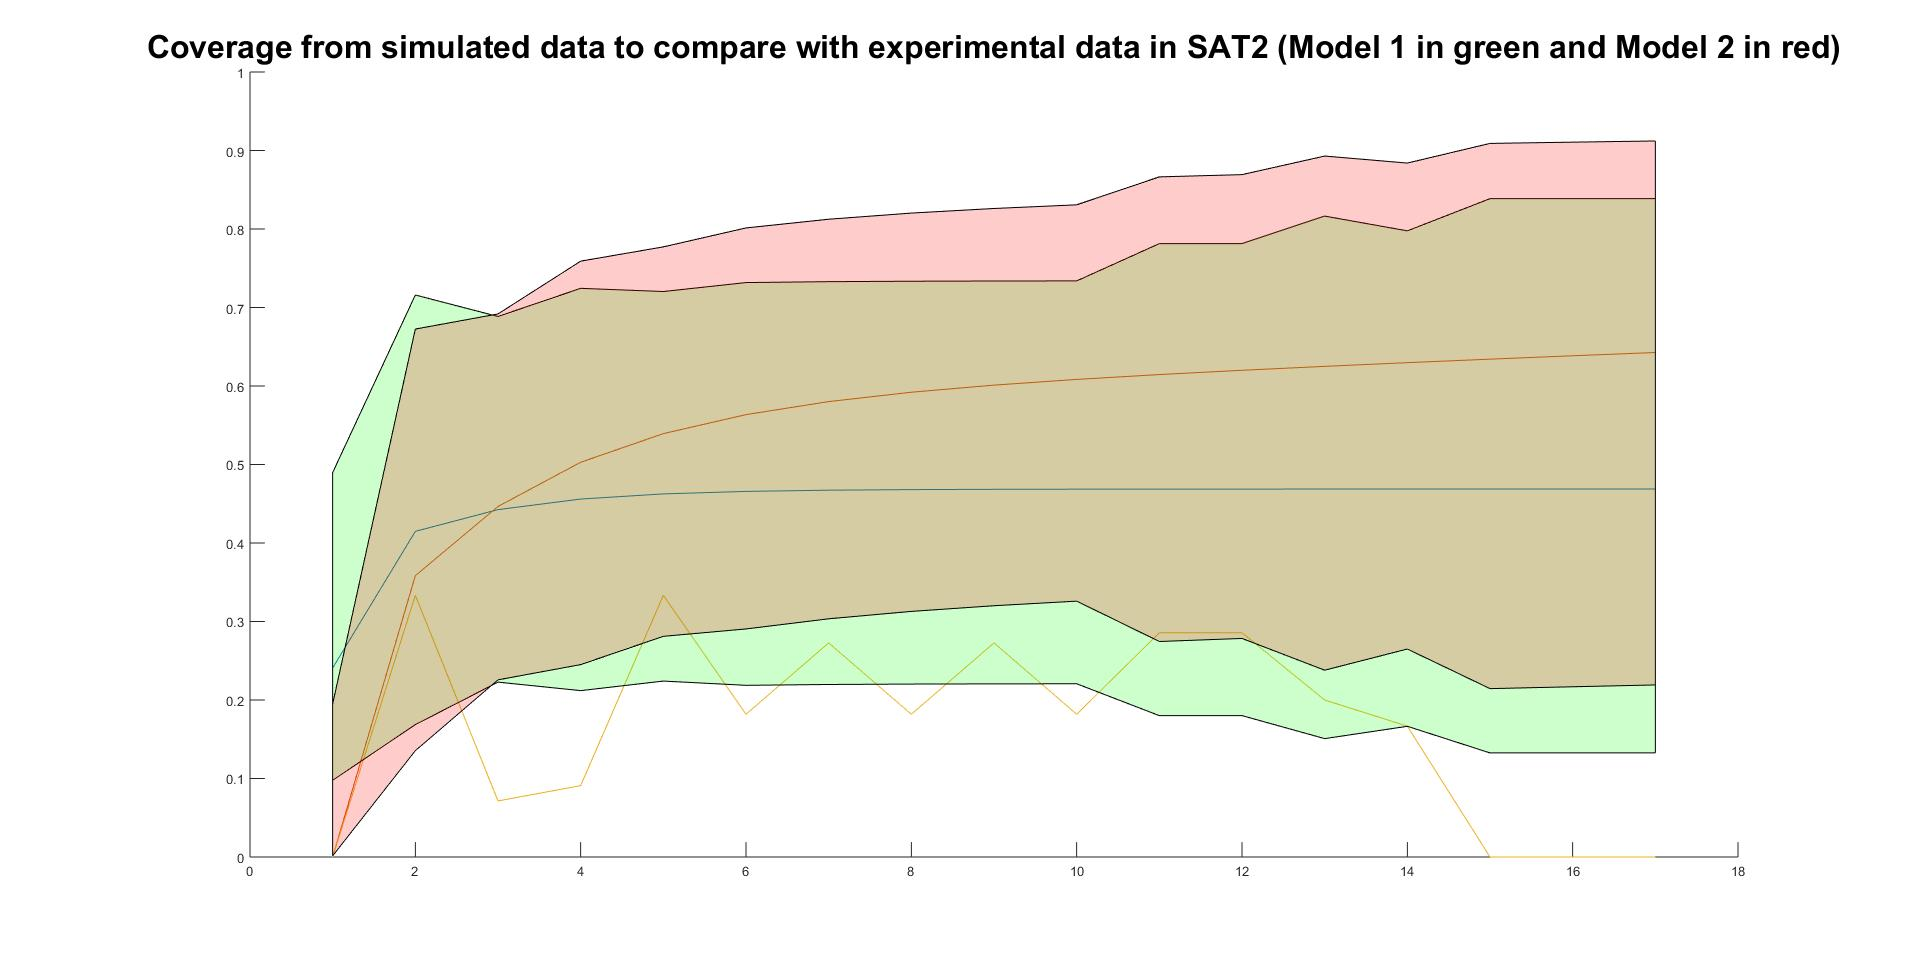
\includegraphics[width=0.4\textwidth]{fig15.jpg}
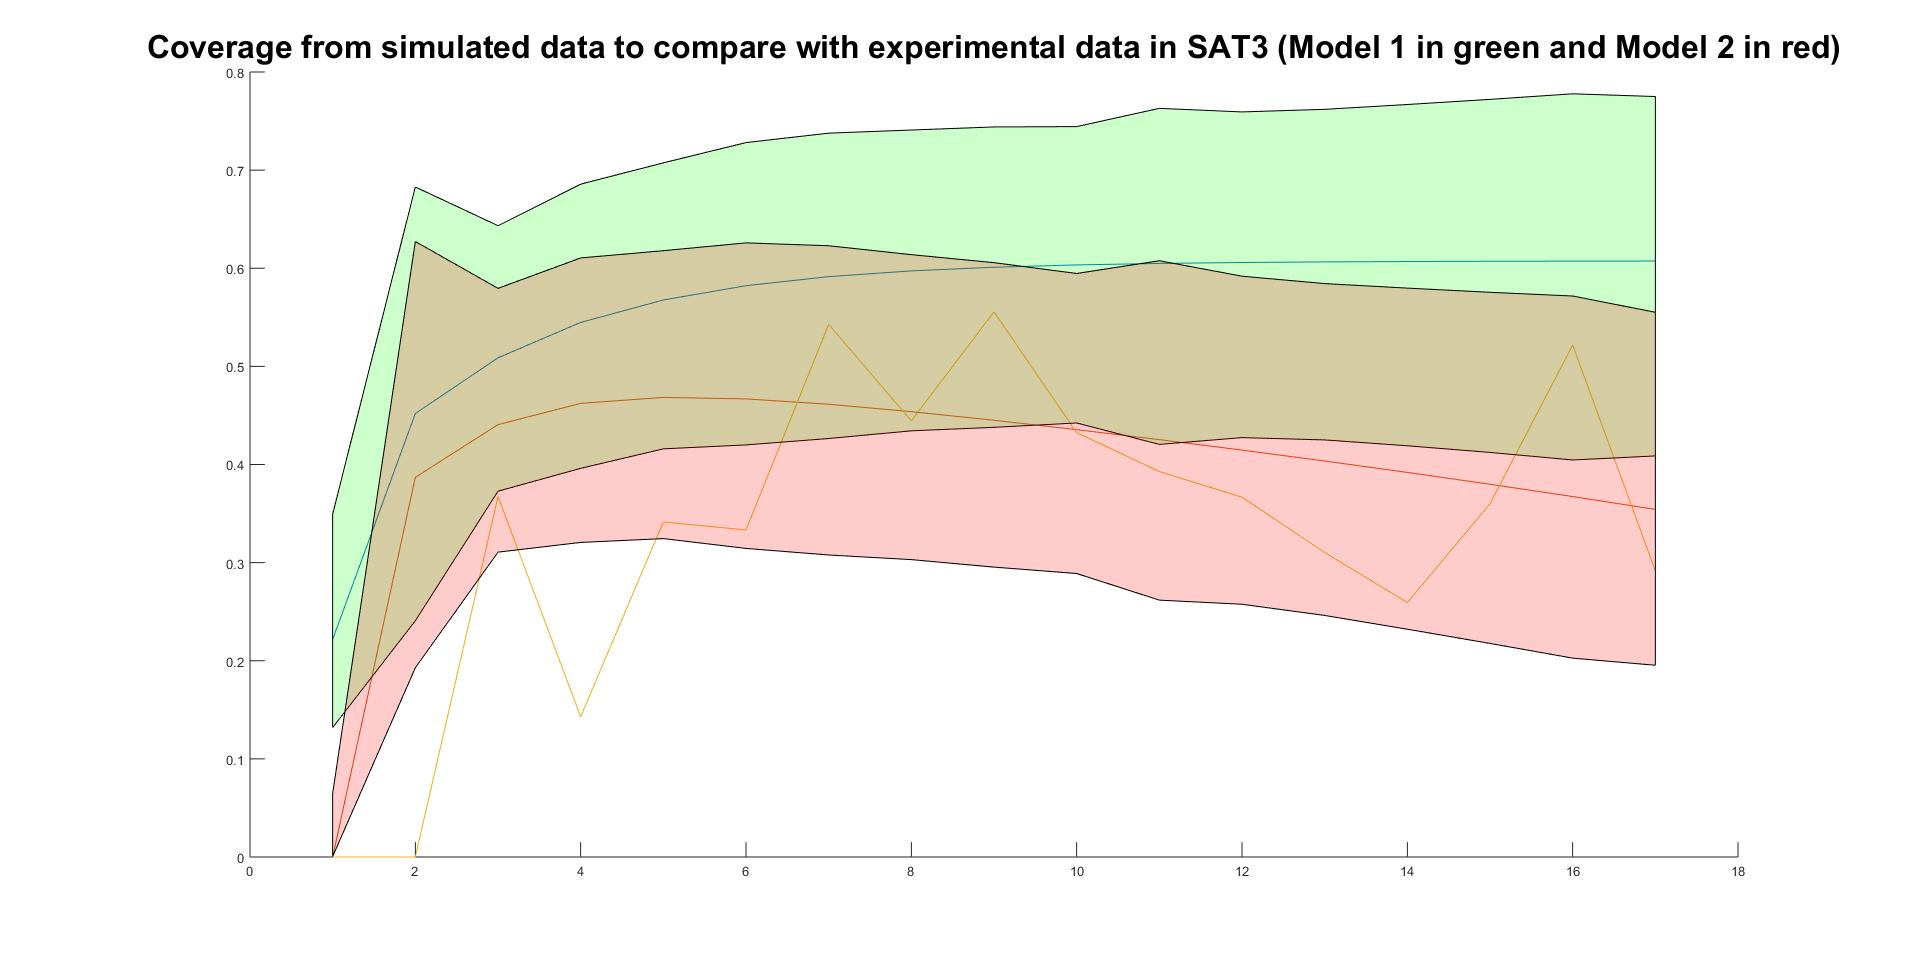
\includegraphics[width=0.4\textwidth]{fig16.jpg}
\end{center}
For SAT1 we have the following results of our MCMC simulations
\begin{center}
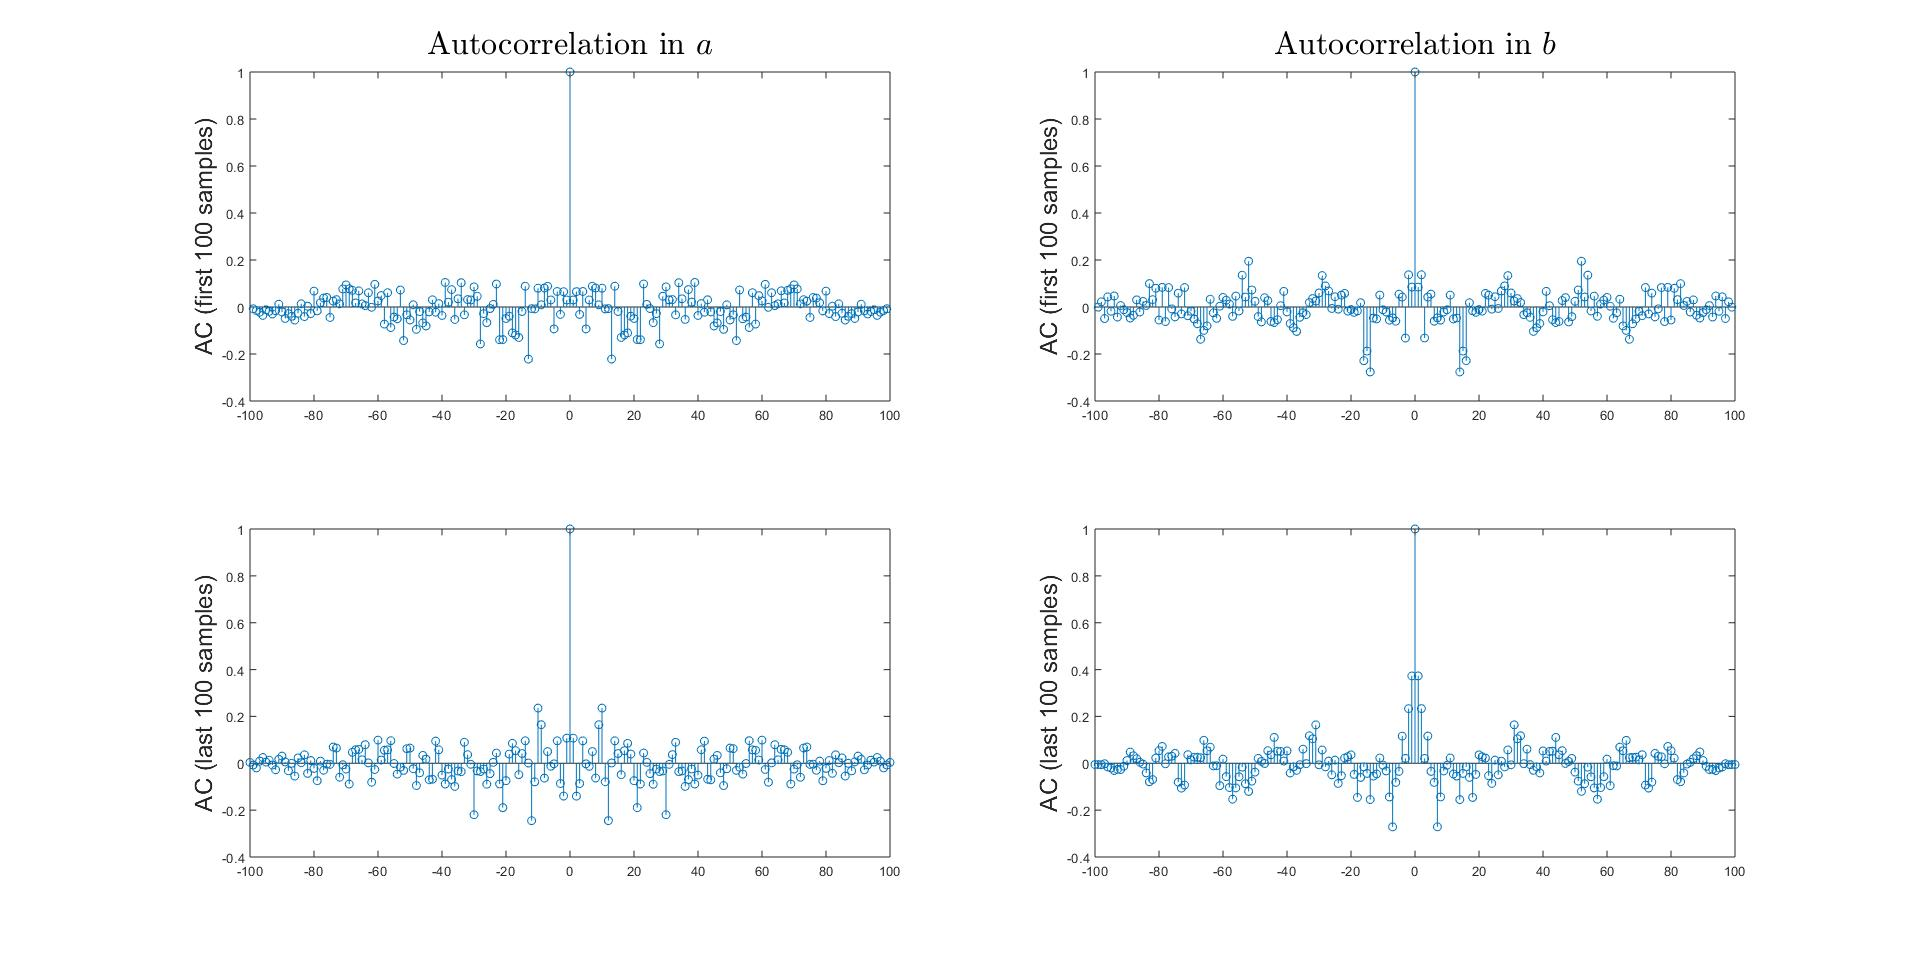
\includegraphics[width=0.4\textwidth]{mcmchcfig1.jpg}
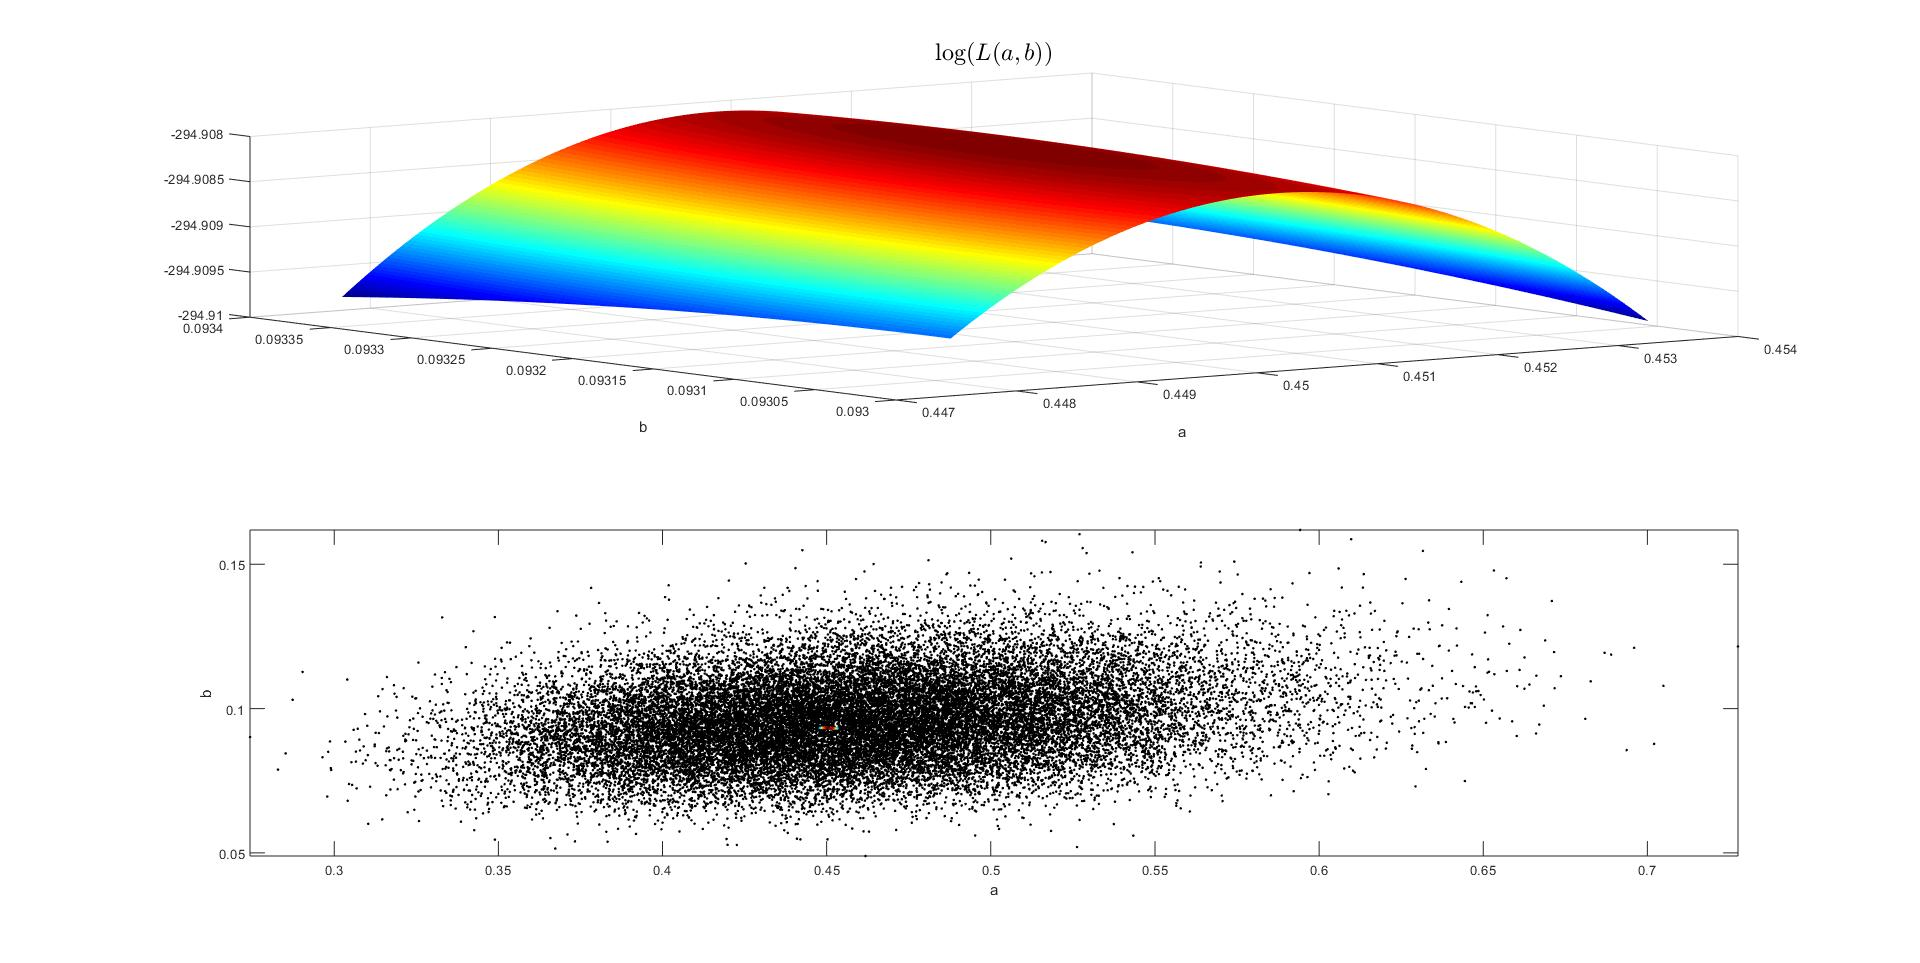
\includegraphics[width=0.4\textwidth]{mcmchcfig2.jpg}
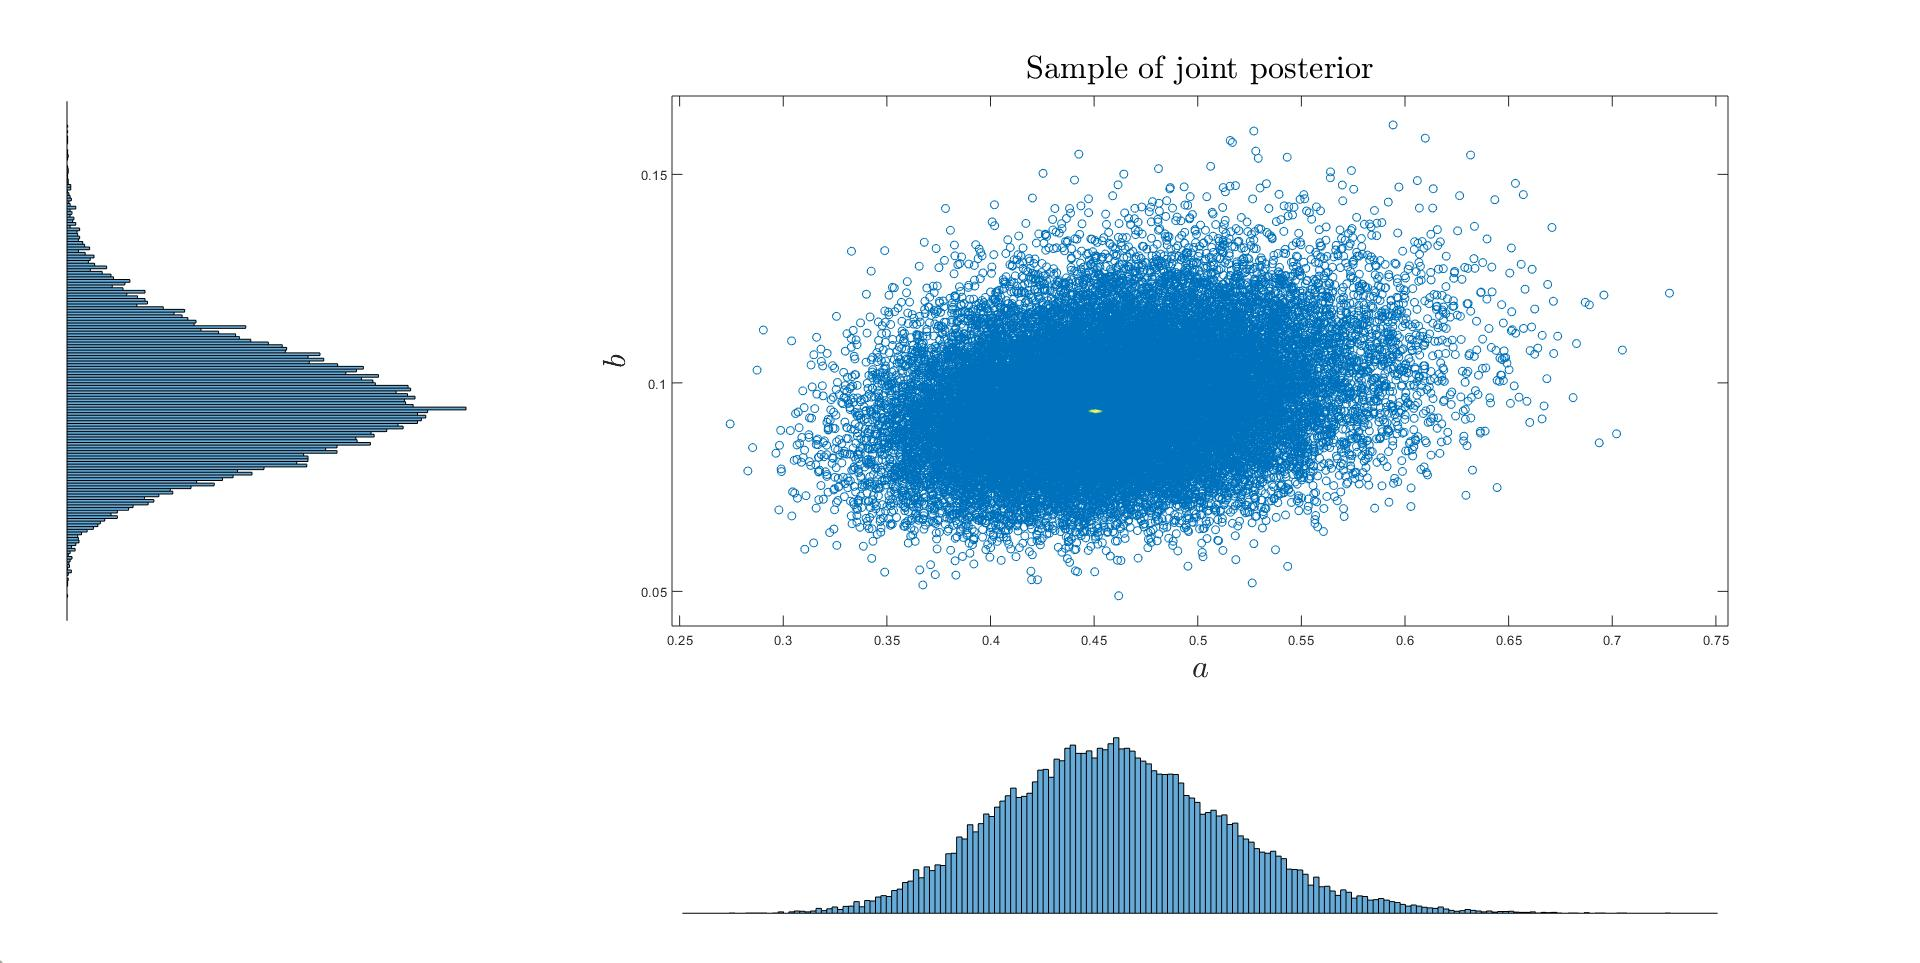
\includegraphics[width=0.4\textwidth]{mcmchcfig4.jpg}
\end{center}
the histogram of the posterior for SAT2 and SAT3
\begin{center}
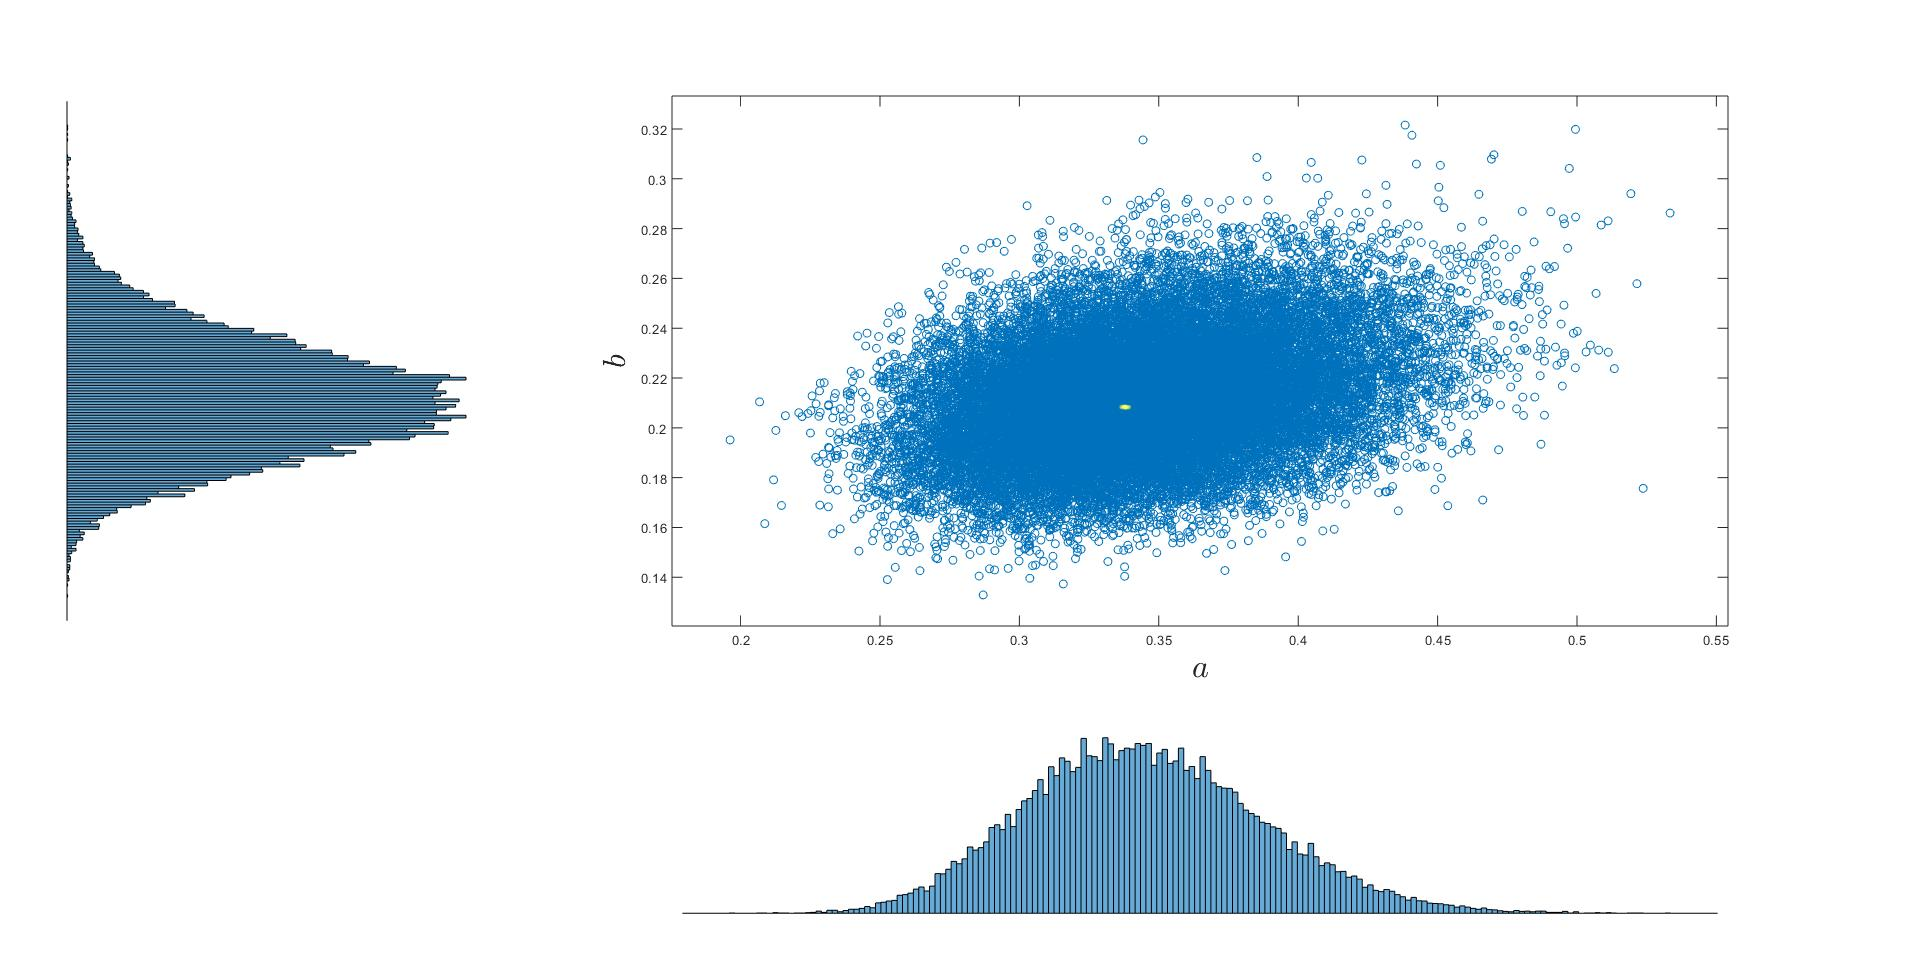
\includegraphics[width=0.4\textwidth]{mcmchcfig8.jpg}
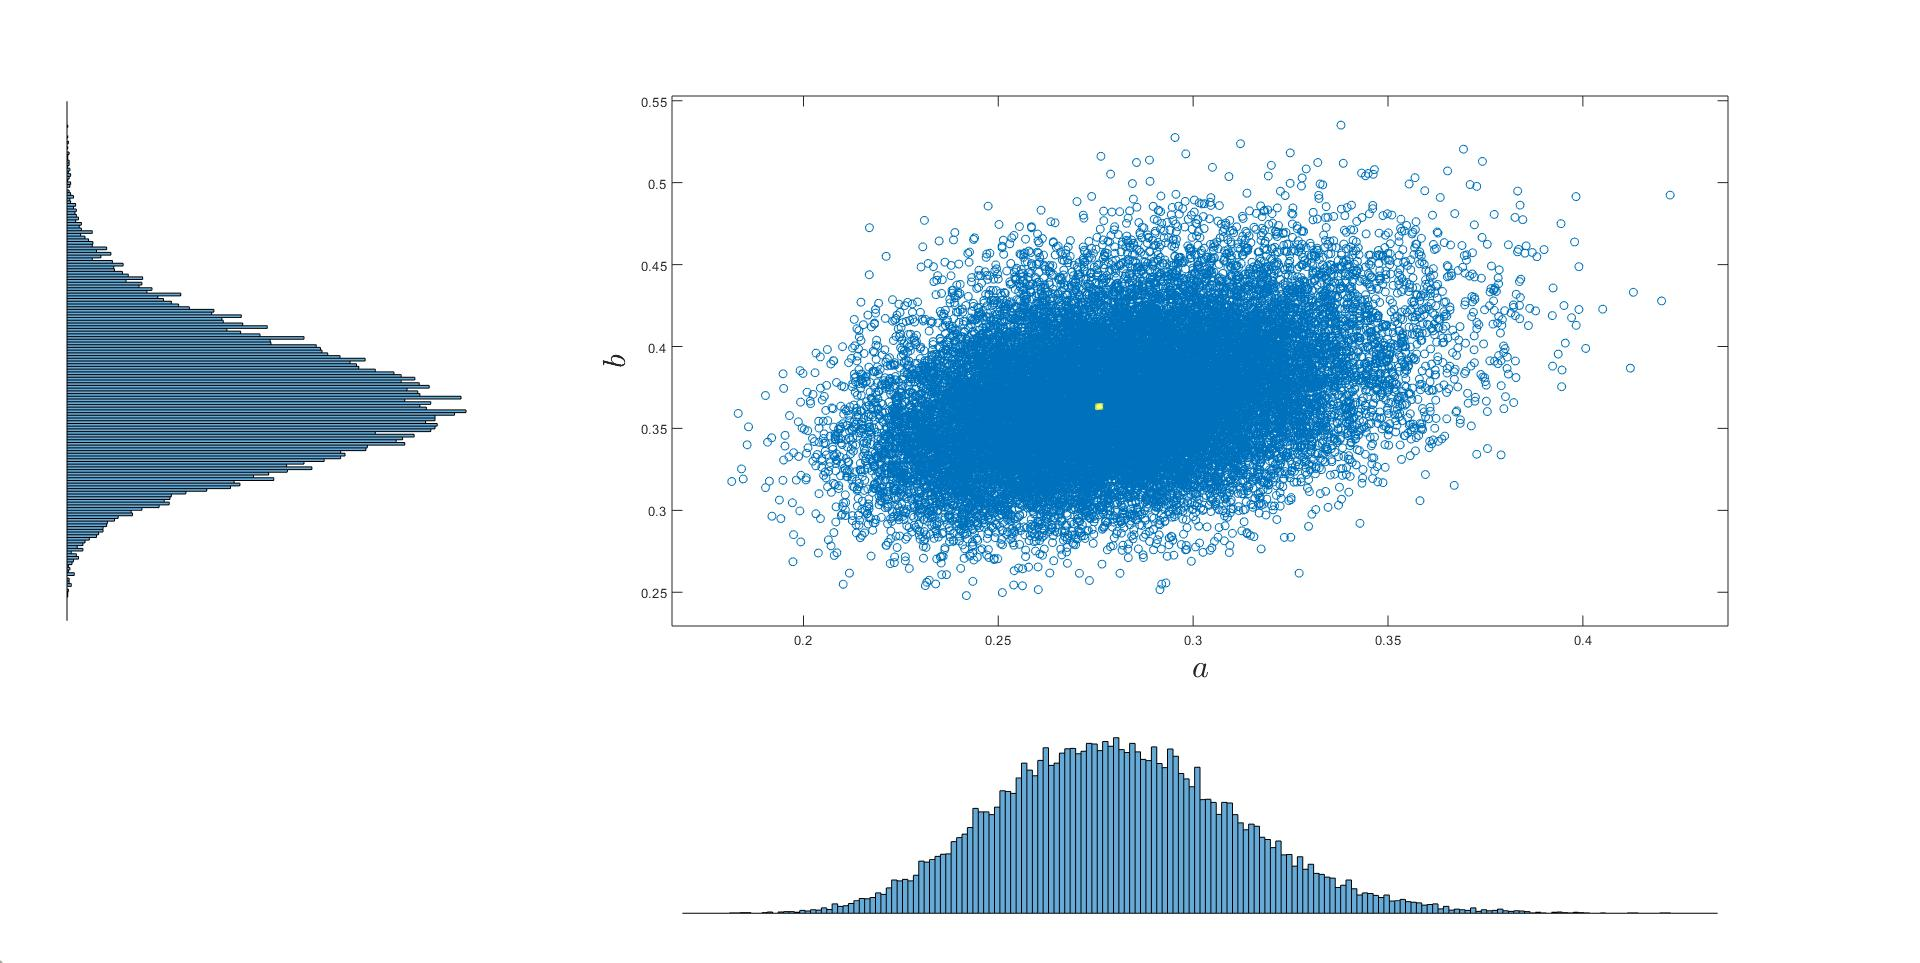
\includegraphics[width=0.4\textwidth]{mcmchcfig12.jpg}
\end{center}
the traceplot of the Markov chain among the different serotypes.
\begin{center}
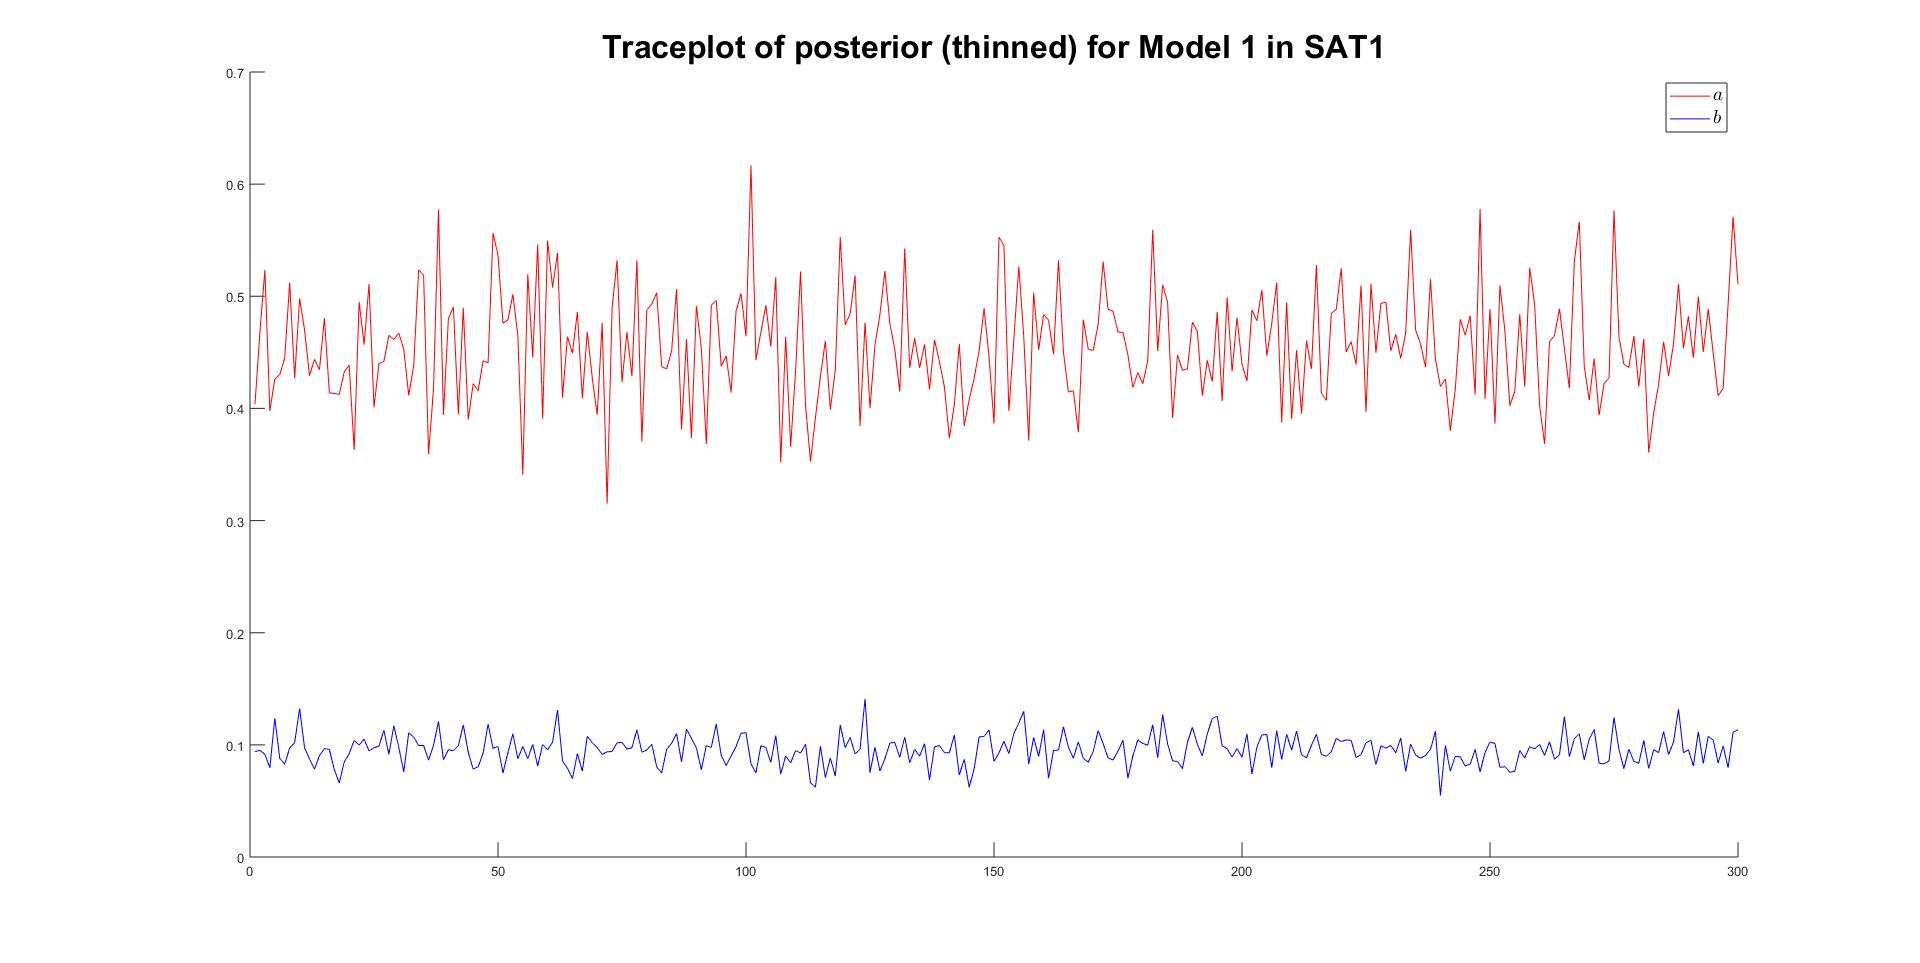
\includegraphics[width=0.4\textwidth]{traceplot1.jpg}
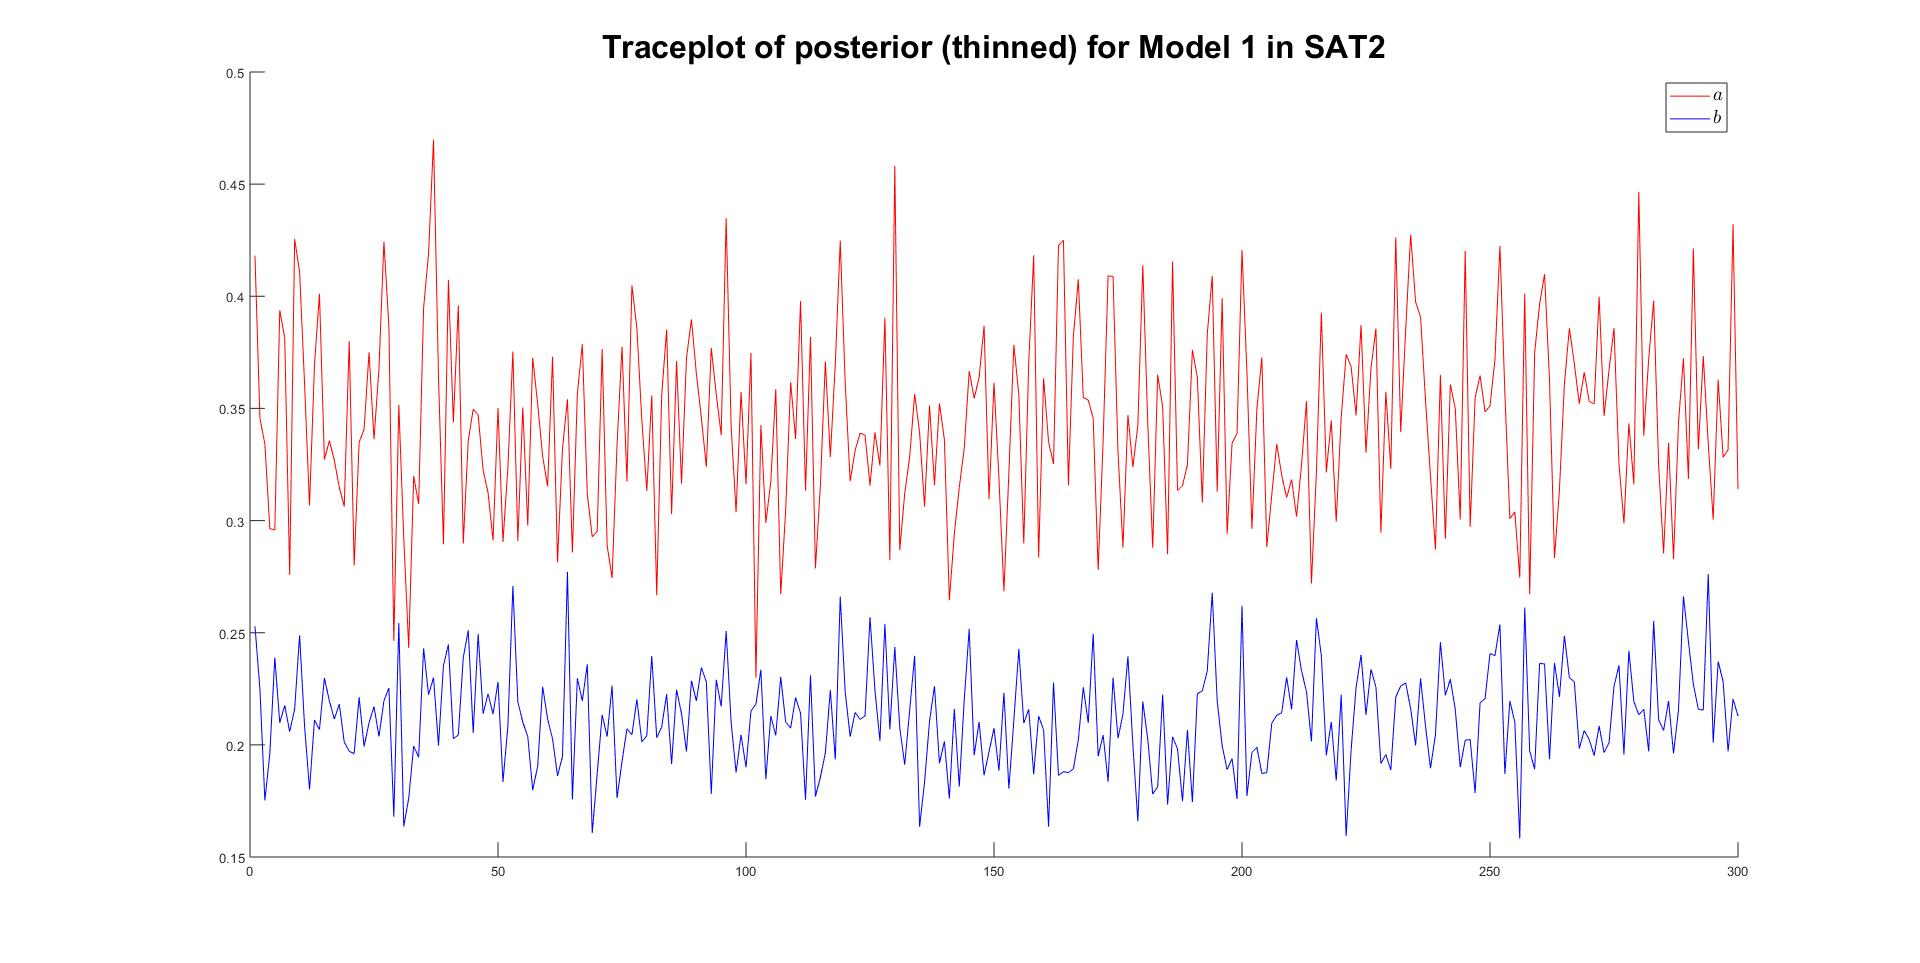
\includegraphics[width=0.4\textwidth]{traceplot2.jpg}
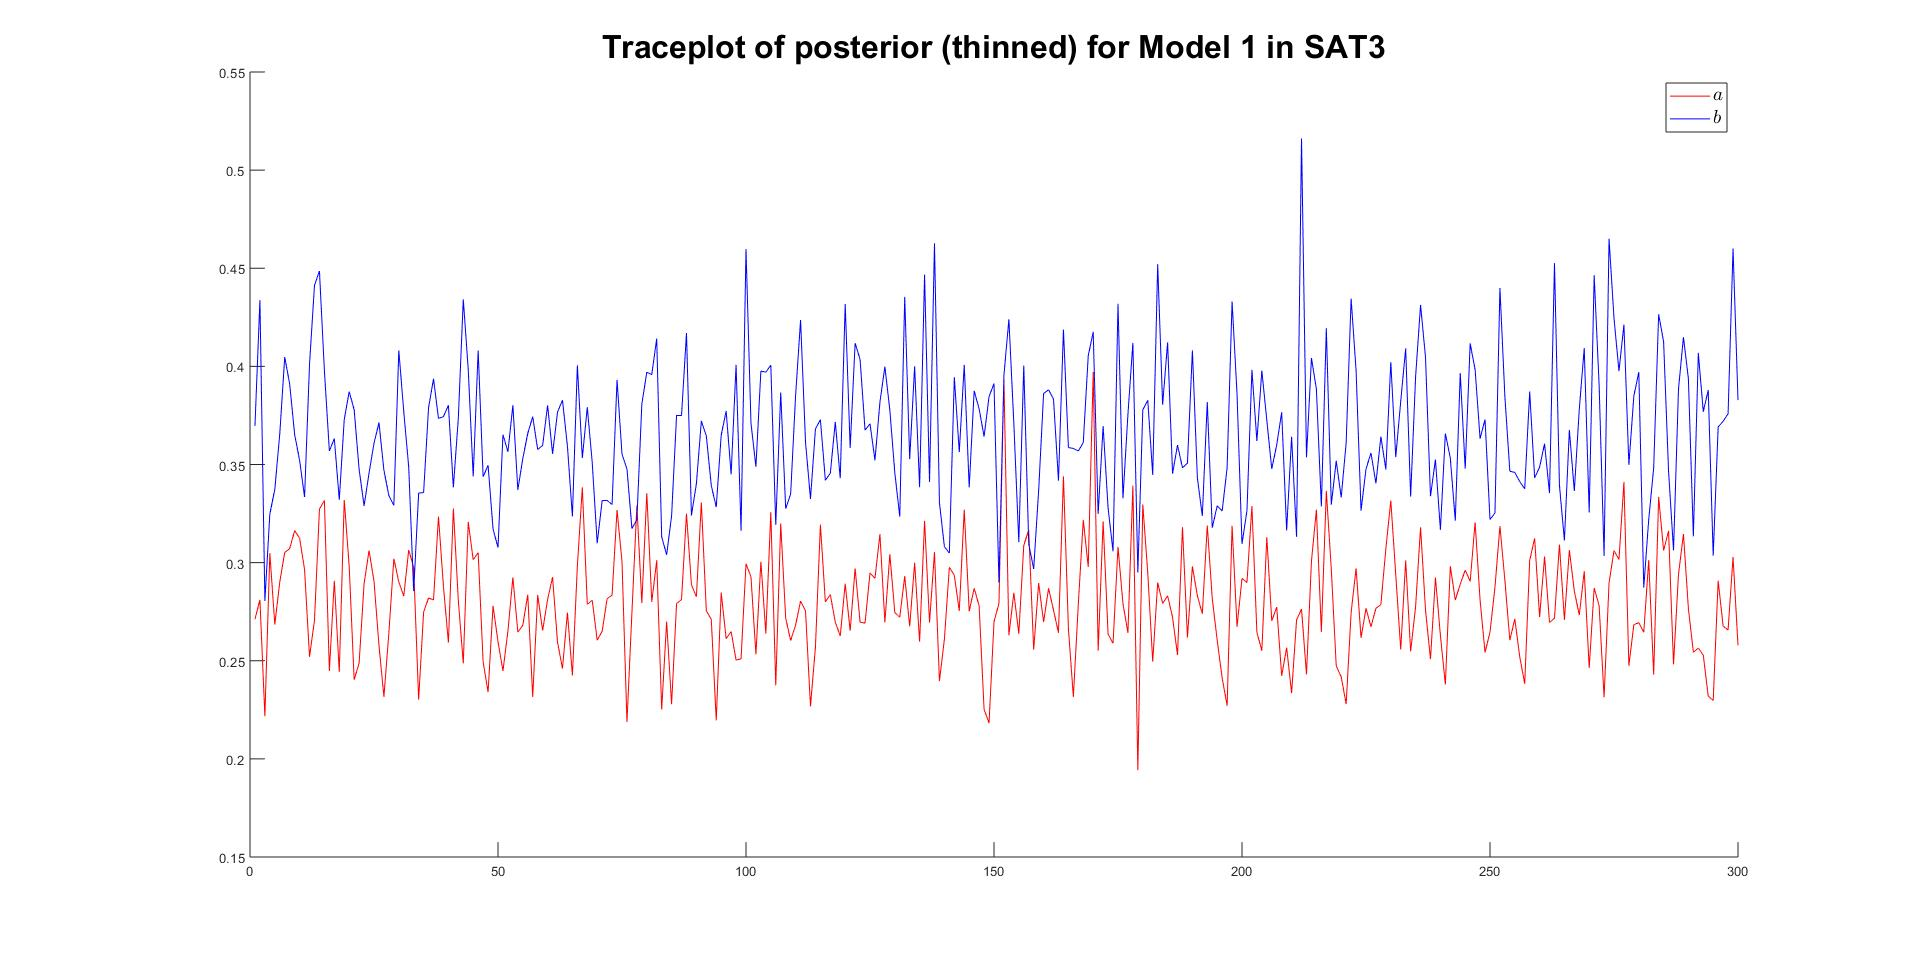
\includegraphics[width=0.4\textwidth]{traceplot3.jpg}
\end{center}
For further information of the set of codes used on this project can be found in 
\url{https://github.com/ricardoreyesgrimaldo/FMDV-immunity}
\end{document}